%\documentclass{cumcmthesis}
\documentclass[withoutpreface,bwprint]{cumcmthesis} %去掉封面与编号页,电子版提交的时候使用。
\usepackage{graphicx} 
\usepackage{cases}
\usepackage{longtable}
\usepackage{float}
%\usepackage{subfigure}
%\usepackage{subfig}
\usepackage{algorithm}
\usepackage{algpseudocode}
\usepackage{threeparttable}
\usepackage{verbatim}
\usepackage[framemethod=TikZ]{mdframed}
\usepackage{url}   % 网页链接
\usepackage{subcaption} % 子标题
\usepackage{makecell}
\usepackage{cleveref}
\usepackage{xcolor}
\usepackage{pgfplotstable} %csv2latex
\usepackage{longtable}

\definecolor{comment_color}{RGB}{85, 139, 78}
\definecolor{string_color}{RGB}{206, 145, 108}
\definecolor{keyword_color}{RGB}{155, 89, 182}
\definecolor{number_color}{RGB}{136, 198, 190}
\definecolor{constant_color}{RGB}{10, 100, 255}
\usepackage{accsupp}
\newcommand{\emptyaccsupp}[1]{\BeginAccSupp{ActualText={}}#1\EndAccSupp{}}
\usepackage{listings}
\lstset{
    language=python,
    linewidth=0.9\linewidth,
    commentstyle=\color{comment_color},
    keywordstyle=\color{keyword_color},
    stringstyle=\color{string_color},
    numbers=left,
    numberstyle=\tiny\color{number_color},
    emphstyle=\color{constant_color}
    numbersep=5pt,
    frame=single,
    framerule=0pt,
    escapeinside=@@,
    emptylines=1,
    xleftmargin=3em,
    tabsize=4,
    gobble=0,
    morekeywords={import, numpy},
    emph={True, False, None, ,BASIC,SMOKE,DRINK,WINE,MEALS,MEAL,FOODS,FOOD,ACTIVITY,HEALTH,DISEASE,BODY,EVALUATE,  STATISTICS, Person, Persons},
    emphstyle=[1]{\color{constant_color}},
    morekeywords={import,def,break,case,catch,classdef,continue,else,elseif,end,for,function,global,if,otherwise,parfor,persistent,return,spmd,switch,try,while},
}

\title{双目标多层贪心下的生产员工培训与产线分配模型}
\tihao{C}
\baominghao{报名号}
\schoolname{上海交通大学}
\membera{麻家乐}
\memberb{黄天浩}
\memberc{刘  灿}
\supervisor{高晓沨}
\yearinput{2023}
\monthinput{9}
\dayinput{xx}

\begin{document}

    \maketitle
    \topskip
    \topmargin
	\renewcommand{\abstractname}{\Large 摘要\\}
	
	\begin{abstract}
	\normalsize
	本文参考进程调度、贪心算法、规划模型等多种思想,建立了一个基于最短完成时间优先(meonf),结合最大化员工技能提升和最小化订单最小超时总和的\textbf{双目标多层贪心优化模型},为生产企业解决员工流动导致的产能和质量问题。
	
	\textbf{针对问题一},本文借鉴操作系统\textbf{进程调度}算法的思想,结合\textbf{贪心算法},考虑每完成一个订单后,以五种不同的标准选择下一个订单进行处理:最短完成时间优先(msf),最短剩余时间优先(erf),最早完工截止时间、最短完成时间优先(dmsf),最早完工截止时间、最短剩余时间优先(derf),以及最小超时订单数、最小超时订单数及最短完成时间优先(meonf)。然后对不同算法的结果进行比较与分析,发现\textbf{meonf算法}得到的结果最优,总超时时间为2125455分钟。最后对算法给出理论解释,说明其合理性。
	
	\textbf{针对问题二},首先,我们发现不同产线的生产压力明显不同,据此将12条产线分为3类,分别为\textbf{繁忙型产线}、\textbf{空闲型产线}和\textbf{周期型产线}。其次,遵循“生产压力越大的产线分配技能水平越高的员工”的原则,将员工分配到不同的产线,以此为目标建立\textbf{线性整数规划模型}求解最优员工分配矩阵。然后对于周期型产线进行\textbf{二次规划}最后,将员工分配到产线,利用问题一的算法计算,得到最短总超时时间为2125455分钟。
	
	\textbf{针对问题三},基于问题一、二建立一个兼顾员工技能提升和订单最小超时总和的\textbf{双目标优化模型},采用问题二的分配矩阵作为初始方案,随每个时间步长采用\textbf{meonf算法}确定订单选择,并参考空闲工人池,结合\textbf{双目标函数最优化}通过多层贪心不断迭代更新该分配矩阵,最终确定生产员工培训与产线分配模型。
	
	\textbf{针对问题四},考虑到不同时间段内存在员工离职,新员工加入的情况,在问题三的模型上针对不同时间段进行\textbf{双目标函数参数的调整},使得特定时间段对关键员工技能水平提升的考虑权重加大,能够适应员工的离职和新员工的培训目标。然后通过分配和培训结果分析该方案的合理性。
	
	\textbf{关键字}:\textbf{贪心算法} \quad \textbf{参数调整} \quad  \textbf{线性整数规划} \quad \textbf{双目标优化}\quad
\end{abstract}



	\section{问题背景与重述}

\subsection{问题背景}
对于以装配测试为主的生产型企业,员工的技能水平是影响生产的一项重要因素。但是,受到复杂因素的影响,员工的流动往往较为频繁,而新员工入职后需要经过专业培训才能进入产线工作,因此在新老员工交替阶段,产线的产能和产品质量往往会产生较大的波动,进而可能会导致严重的后果。该问题可以通过恰当的员工管理和产线分配策略解决。

\subsection{问题提出}
现有某生产企业40天内的生产订单数据、20名员工具体的技能水平数据和新员工的培训要求,要求对目前对生产员工培训与产线分配的策略提出优化方案,使得产能在员工流动时保持基本的稳定,新员工可以无缝地加入后续生产队列。问题的设置是逐渐加强限制条件,并服务于同一主题的:

\begin{enumerate}[label=(\arabic*)]
    \item \textbf{问题一}:在企业存在足够多员工、员工在所有产线上的技能水平均为 E、不考虑培训与升级的情况下,设计最优分配方案,使得所有订单的超时分钟数之和最小,并给出超时分钟数之和。
    \item \textbf{问题二}:在员工数量有限、员工技能水平存在差异、员工不能进行培训与升级、员工无增减变化的情况下,重复问题一的任务。
    \item \textbf{问题三}:在员工数量有限、员工技能水平存在差异、员工可以培训升级、员工无增减变化的情况下,重复问题一二的任务,使得完成订单的同时尽可能提升员工的技能水平(必要时可适当牺牲一些超时分钟数),并给出最优的培训方案。
    \item \textbf{问题四}:在问题三的生产计划分配的基础上,假设在第2250分钟,员工PE001到PE010提出离职申请,并在第4500分钟离职,同时在第6750分钟,10名新员工将入职,其所有技能水平均为N。给出相对较优的生产计划调整方案,使得所有订单的超时分钟数之和最小,说明方案的合理性,并给出超时分钟数之和。
\end{enumerate}
	\section{数据预处理}

考虑到本题数据的特殊性,我们需要讨论产线、订单、产品、员工之间的关系,因此在数据处理前我们设计了LINE、ORDER、PRODUCT、WORKER四个基本类,用来记录和管理本题的数据,下表是我们对这些类的设计。

\begin{table}[!ht]
    \caption{类的设计详细介绍}
    \centering
    \begin{tabular}{c@{\hspace{20pt}}c@{\hspace{20pt}}c@{\hspace{20pt}}c}
    \toprule[1.5pt]
    符号     & 名称       & 内容         \\ \hline 
    LINE     & 产线   & 工作订单,等待队列,阻塞队列等   \\ \hline
    ORDER    & 订单   & 产品队列,分配员工,截止时间等   \\ \hline
    PRODUCT  & 产品   & 标准工时,产品数量,分配员工,产线名称等  \\ \hline
    WORKER   & 员工   & 技能水平,训练时长,培训情况等   \\ 
    \bottomrule[1.5pt]
    \end{tabular}
\end{table}













	\section{符号和变量说明}

\begin{center}

    \begin{tabular}{c@{\hspace{50pt}}c}
    	\toprule[2pt]  %添加表格头部粗线
    	符号或变量    &    意义\\
    	\midrule[1pt]  %添加表格中横线
        $m_{ij}$        & 员工$i$对产线$j$的技能水平 \\
        $Level_{k-j}$         & 员工k对产线j的技能 \\
        $E_{j}$         & 产线$j$工位数 \\
        $Group_i$         & 第i个可分配员工组合 \\
        $impro_i$         & 第i个可分配员工组合的技能提升正价值 \\
        $badtime_i$         & 第i个可分配员工组合的超时负价值 \\
        $Workers_i$         & 第i个可分配员工组合的员工集 \\
        $pracimpro_k$         & 员工k的实践提升水平 \\
        $theomiss_k$         & 员工k的理论提升水平 \\

        $ratiop_m$         & m类技能水平员工的实践提升系数 \\
        $ratiot$         & 理论提升系数 \\
        
        
    	\bottomrule[1.5pt] %添加表格底部粗线
	\end{tabular}
	
\end{center}  \hspace*{\fill}

注:其他符号将在文中具体说明
    \section{模型假设}
\begin{enumerate}
    \item 为方便分析,结合现实逻辑,认为新员工必须先完成理论培训才能进行产线培训。
    
    \item 对于每个订单,只分配一次员工和培训情况,并且认为被分配到的员工始终进行生产直到该订单所有产品生产完成。
    
    \item 考虑员工升级的时候,认为员工技能等级的提升优先于员工经验值的累计,为其分配一个更大的系数。
    
    \item 离职的员工会把当前分配到的订单完成后再离职。
\end{enumerate}


    \section{问题分析}

\subsection{问题一分析}
本问题情景类似于操作系统的进程调度。我们采用\textbf{贪心}的思想,考虑每完成一个订单后,以五种不同的标准选择下一个生产的订单:完成时间最短优先,剩余时间最短优先,完工截止时间最早、完成时间最短优先,完工截止时间最早、剩余时间最短优先,以及超时订单数最小、完成时间最短优先。比较所有算法结果的优劣,并从理论上给出合理的解释。

\subsection{问题二分析}
由于每条产线在做每个订单、每件产品在生产的时候员工不能替换,因此考虑将员工分配到不同的产线,再采用问题一的最优算法meonf计算得到总超时时间。经过问题一的分析,发现某些产线生产压力较大,超时现象难以避免,而另外一些产线生产压力较小,几乎不存在超时的问题。因此,为了最小化总超时时间,分配员工时应尽量使得生产压力越大的产线分到的员工技能水平越高。以此为目标建立\textbf{线性整数规划模型},求解最优员工分配矩阵。


\subsection{问题三分析}
本题在前述问题的基础上增加一条“员工可以培训升级”的条件。根据题意,我们需要同时考虑尽可能提升员工技能水平和最小化总超时时间两个目标,因此在问题一和问题二的基础上建立\textbf{双目标优化模型},并将问题二的分配矩阵作为初始方案,利用\textbf{贪心}的思想,设计了算法进行求解。

\subsection{问题四分析}
由于存在员工流动的情况,考虑根据关键时间点将时间分段,不同时间段内根据员工生产情况对问题三的双目标函数参数进行调整,使得特定时间段对关键员工技能水平提升的考虑权重加大,保证生产进度的稳定性。	
    \section{问题一的模型建立与求解}
对于本问题情景,采用\textbf{贪心}的思想,参考操作系统进程调度的几种算法,考虑每完成一个订单后,如何选择下一个生产的订单,以达到总超时时间最小的目标。下面设计5种选择标准,形成5种算法进行求解:完成时间最短优先,剩余时间最短优先,完工截止时间最早、完成时间最短优先,完工截止时间最早、剩余时间最短优先,以及超时订单数最小、完成时间最短优先。所有算法的具体代码见附录。相应名词解释如下:
\begin{itemize}
    \item \textbf{完成时间}(\verb|sum_time|):完成订单所需要的时间,由每件产品的标准工时以及订单内容计算得到。
    \item \textbf{剩余时间}(\verb|rm_time|):若选择某订单,完成该订单后距离完工截止时间所剩的时间。
\end{itemize}

      \subsection{最短完成时间优先(msf)}
      本算法意在每次选择完成最快的订单作为下一个生产订单,以最小化平均等待时间或完成时间。最终所得总超时时间为2928861分钟。
      
      本算法的问题很明显,就是完成时间长的订单可能会一直等待,导致饥饿问题,使得超时时间过大。因此,本算法主要作为其他算法结果的参考。
      
      \subsection{最短剩余时间优先(erf)}
      本算法的核心思想是在多个待生产的订单中选择最紧迫的订单先完成,以解决长订单饥饿的问题,达到更优的公平性。
      最终所得总超时时间为2678287分钟。
      
      \subsection{最早完工截止时间、最短完成时间优先(dmsf)}
      针对最小化总超时时间的目标,采用\textbf{双贪心}策略,在mlf的基础上添加一个更高优先级的选择标准:完工截止时间最早,即根据完工截止时间将时间分段,在每段里优先生产短订单。
      最终所得总超时时间为2362896分钟。
      \subsection{最早完工截止时间、最短剩余时间优先(derf)}
      采用dmlf相同的思想,但在每个时间段里优先选择最紧迫的订单。
      最终所得总超时时间为2514299分钟。
      
      \subsection{最小超时订单数、最短完成时间优先(meonf)}
      采用\textbf{双贪心}策略。算法的核心思想是在每个完工截止时间到来时,选择使得超时订单最少的订单进行处理。第二贪心目标是订单的生产时间,即多个订单的最小期望超时数量相同时,短订单优先。
      最终所得总超时时间为2125455分钟。
      
      \subsection{结论与分析}
      最终meonf算法所得总超时时间最小,为2125455分钟。具体分配方案见附录\cref{tab:problem1}。下面从两个角度给出合理性解释。
      
      \subsubsection{最短完成时间优先}
      在每个完工截止时间即将到来时,可以证明,\textbf{将订单按所需生产时间从小到大的顺序处理,所得收益最大}。
      
      假设有一系列订单,编号为$1,2,\ldots,k,k+1$,每个订单的所需的生产时间为$a_1,a_2,\ldots,\\a_k,a_{k+1}$,其中$a_1 < a_2 < \cdots < a_k < a_{k+1}$。现将订单按所需生产时间从小到大排序,如\cref{fig:p1}所示。现在即将到达一个截止时间$t$,使得$k-1$号订单正好超时。此时的超时分钟数之和为
\begin{equation}
    \label{eq:p1} 
    T_1=3(a_1+a_2+\cdots+a_{k-1}-t)+2a_k+a_{k+1}
\end{equation}
      
\begin{figure}[h]
    \centering
    \begin{minipage}[c]{0.3\textwidth}
        \centering
        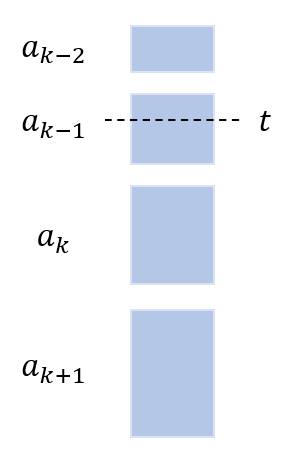
\includegraphics[height=0.2\textheight]{pics/p1.png}
        \subcaption{顺序排序}
        \label{fig:p1}
    \end{minipage} 
    \begin{minipage}[c]{0.3\textwidth}
        \centering
        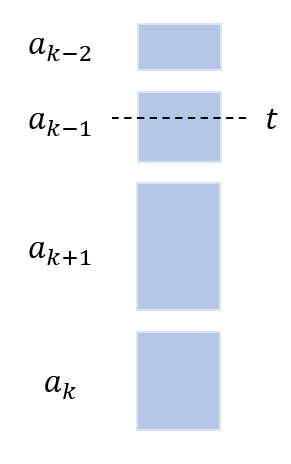
\includegraphics[height=0.2\textheight]{pics/p2.png}
        \subcaption{情况一}
        \label{fig:p2}
    \end{minipage} 
    \begin{minipage}[c]{0.3\textwidth}
        \centering
        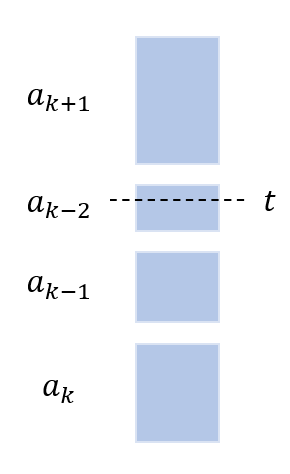
\includegraphics[height=0.2\textheight]{pics/p3.png}
        \subcaption{情况二}
        \label{fig:p3}
    \end{minipage} 
  \caption{不同订单处理顺序示意图}
  \label{fig:pro1}
\end{figure}
      
      若不按订单按所需生产时间从小到大排序处理,考虑将$k+1$号订单前移。可能有以下2种情况:
      
      \textbf{情况一}:若移动后的$k+1$号订单仍然超时,如\cref{fig:p2}所示。此时的超时分钟数之和为
\begin{equation}
    \label{eq:p2} 
    T_2=3(a_1+a_2+\cdots+a_{k-1}-t)+2a_{k+1}+a_k
\end{equation}

\cref{eq:p2}减去\cref{eq:p1},由于$a_k < a_{k+1}$,因此有
\[T_2-T_1=a_{k+1}-a_k>0\]

即总超时时间比顺序处理长。若移动后$k+1$号订单部分在截止时间内,类似可证超时时间增加。

\textbf{情况二}:若移动后的$k+1$号订单未超时,如\cref{fig:p3}所示。此时的超时分钟数之和为
\begin{equation}
    \label{eq:p3} 
    T_3=3(a_1+a_2+\cdots+a_{k-2}+a_{k+1}-t)+2a_{k-1}+a_k
\end{equation}

\cref{eq:p3}减去\cref{eq:p1},由于$a_{k-1} < a_k < a_{k+1}$,因此有
\[T_3-T_1=2a_{k+1}-a_k-a_{k-1}>0\]

即总超时时间比顺序处理长。其他情况均类似可证,在此不一一列举。因此,将长订单前移将增大总超时时间,故考虑将订单按所需生产时间从小到大的顺序处理具有合理性。
      
      \subsubsection{最小超时订单数优先}
       每次选择下一份订单时希望造成的超时订单数最少,是因为每多一个超时的订单,计算总超时时间的时候就要多一个累加对象,在短期看来效益较差。
    \section{问题二的模型建立与求解}

\subsection{产线特性分析}
对于每条产线,我们都统计了其在所有订单所需总时长之和(假设所有工人的技能水平均为E),并将其与该产线所有订单的最晚截止时间作比较,结果如下表:
\begin{table}[htbp]
    \caption{产线特性分析}
    \label{tab:workline} 
    \centering
    \begin{tabular}{@{\hspace{10pt}}cccc@{\hspace{10pt}}}
        \toprule[1.5pt]
        产线 & 所有订单总耗时 & 最晚截止时间 & 与最晚截止时间的差值\\
        \midrule[1pt]
        line1  & 670 & 18000 &  -17330 \\
        line2  & 27897 & 18000 & 9897          \\
        line3  & 26992 & 18000 & 8992         \\
        line4  & 33035 & 18000 & 15035         \\
        line5  & 7159 & 18000 & -10841      \\
        line6  & 3778 & 18000 &  -14222  \\
        line7  & 34961 & 18000 &  16961 \\
        line8  & 11687  & 13000 &  -1323\\
        line9  & 4400   & 18000 & -13600 \\
        line10 & 35251 &  18000 &     17251\\
        line11 & 15200  & 18000 &     -2800 \\
        line12 & 5943   & 18000 & -12057\\ 
        \bottomrule[1.5pt]
    \end{tabular}
\end{table}

对于这11条产线,可以分为以下三种:
\begin{itemize}[left=1em]
    \item \textbf{繁忙型产线} :与最晚截止时间的差值接近或超过10000(如产线2,3,4,7,10),这意味着平均有几十个订单一定会超时,其降低分配工人的生产能力对超时总时间的影响是巨大的。且对于这类产线而言,总时长越长意味着全程的压力越大,因此应该在整个过程中分配尽量多技能水平为E的工人且不发生改变。
    \item \textbf{空闲型产线} :与最晚截止时间差值很小,小于 -10000 (如产线1,5,6,9,12)。对于这类产线,进一步分析可以发现其在每个截止时间内所有订单总耗时之和均不会超时,意味着该产线的工人长期处于空闲阶。对于这类产线总时长越短表示全程的压力越小。因此可以分配能力为O的工人且适合进行产线培训(针对第三问)。
    \item \textbf{周期型产线} :总时长略小于最晚截止时间(在- 5000以内)(产线8,11)。这类产线存在不同截止日期内订单的超时情况不同,主要体现为最终不超时但局部超时。对于这些产线,在不同的时间段需要调整其工人分配策略,如在其局部超时的时候,需要为其尽量分配能力为E的工人。
\end{itemize}


易知,这三种类型的产线切换不同能力等级的工人产生的影响大小为:繁忙型产线>周期型产线>空闲型产线。可以看到,他们的所有订单总耗时存在明显的差别。


\subsection{模型建立}
\subsubsection{线性0-1规划模型}
\textbf{确定决策变量}:问题需要求得最优的员工分配策略,因此本模型的决策变量应为每位员工分配产线的情况。引入0-1变量表示如下:
\begin{equation}
    \label{eq:01}
    x_{ij}=
    \begin{cases}
        1 & \text{工人}i\text{分配到产线}j \\
        0 & \text{工人}i\text{未分配到产线}j
    \end{cases}
\end{equation}

\textbf{确定优化目标}:模型需要尽量将技能水平高的员工分配到生产压力大的产线。令$T_j$表示产线$j$生产完毕所有订单所需的总时长,则$\frac{T_j}{\sum_j T_j}$定量衡量了每条产线的生产压力大小。优化目标为:
\begin{equation}
    \label{eq:goal}
    \max \sum_{ij} \frac{T_j}{\sum_j T_j} m_{ij}x_{ij}
\end{equation}

\textbf{确定约束条件}:由每条产线的工位数限制,有
\begin{equation}
    \label{eq:i}
    \sum_i x_{ij} \leq E_j ,\quad \forall j
\end{equation}

因每位员工一次只能分配到一条产线工作,故有
\begin{equation}
    \label{eq:j}
    \sum_j x_{ij} \leq 1 ,\quad \forall i
\end{equation}

综上,员工分配线性规划模型为:
\[
    \max \sum_{ij} \frac{T_j}{\sum_j T_j} m_{ij}x_{ij} 
\]
\[
    s.t.
    \begin{cases}
        \sum_i x_{ij} \leq E_j ,\quad \forall j \\
        \sum_j x_{ij} \leq 1 ,\quad \forall i
    \end{cases}
\]

\subsection{模型求解}
模型建立后,编写python程序,调用PuLP库进行求解,得到分配策略如\cref{tab:workers}所示。

\begin{table}[htbp]
    \caption{问题二员工分配策略}
    \label{tab:workers} 
    \centering
    \begin{tabular}{@{\hspace{40pt}}c@{\hspace{80pt}}c@{\hspace{40pt}}}
        \toprule[1.5pt]
        产线 & 分配员工 \\
        \midrule[1pt]
        line1  & PE002    \\
        line2  & PE009、PE011          \\
        line3  & PE006          \\
        line4  & PE003、PE012、PE015         \\
        line5  & PE016       \\
        line6  & PE018      \\
        line7  & PE005、PE007   \\
        line8  & PE004  \\
        line9  & PE017      \\
        line10 & PE001、PE008、PE010     \\
        line11 & PE014        \\
        line12 & PE013      \\
        \bottomrule[1.5pt]
    \end{tabular}
\end{table}

\subsection{模型优化}

考虑到7.1节中分析的产线情况,对于产线8和产线11,需要根据其局部时间段内的繁忙程度进行工人分配策略的调整。

因此在确定了上述员工分配表后,我们固定其他产线的工人分配结果,对产线8、11在不同截止日期前的分配结果做第二次规划,模型如下:

\[
    \max \sum_{ij} \frac{T_j^{\prime}}{\sum_j T_j^{\prime}}  m_{ij}x_{ij} \quad \quad j = 8,11
\]
\[
    s.t.
    \begin{cases}
        \sum_i x_{ij} \leq E_j ,\quad  j  = 8, 11\\
        \sum_j x_{ij} \leq 1 ,\quad \forall i \\ 
        x_{ij} = y_{ij}, \quad j \neq 8, 11
    \end{cases}
\]

其中$T_j^{\prime}$表示每同一个截止日期下的所需订单总时长,$y_{ij}$表示上述分配结果。

对每一个截止时间进行求解,得到的结果均与原分配策略相同,证明不需要在中途改变员工分配情况。

\subsection{最终结果与分析}
根据\cref{tab:workers}将员工分配到对应产线进行生产,采用问题一的meonf算法得到最终的订单分配结果,结果与问题一相同,如\cref{tab:problem1}所示。最终超时分钟数之和为2125455。
    \section{问题三的模型建立与求解}
本文针对问题三设计了一个兼顾员工技能水平提升和优化最小超时总和的\textbf{双目标优化模型},并采用\textbf{贪心算法}求解。
模型的整体框架图如\cref{fig:stru}:

\begin{figure}[h]
    \centering
    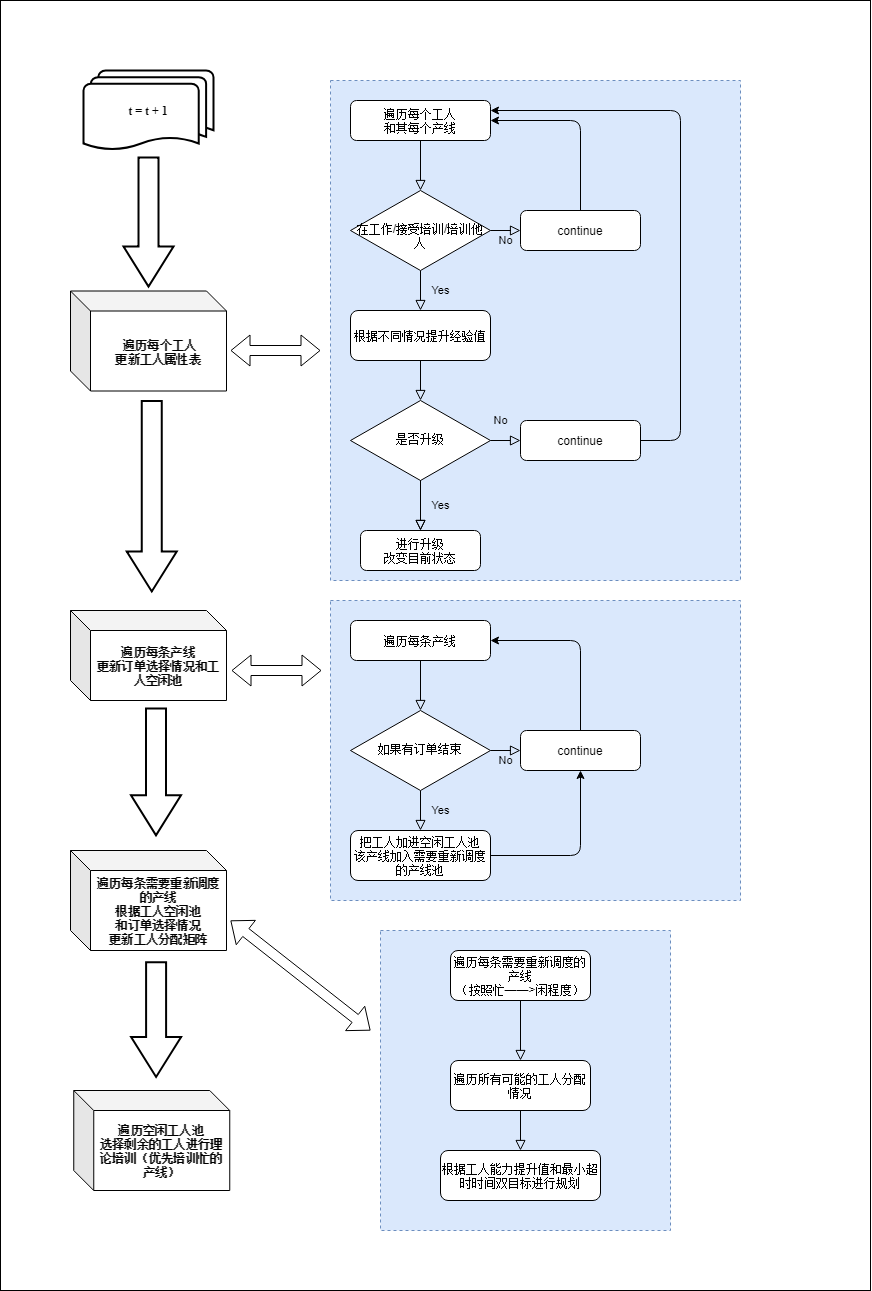
\includegraphics[height = 0.65\textheight]{pics/p4.png}
    \caption{问题三算法结构图}
    \label{fig:stru}
\end{figure}
\newpage

\subsection{员工技能水平更新}
员工技能水平更新发生在每个时间片(min),其根据时间轴的前进更新员工的技能属性指标。我们先介绍员工属性表,然后介绍技能属性的更新策略。

\subsubsection{员工属性设定}
对于每个员工,为其设置以下几个属性:

\begin{table}[htbp]
    \caption{员工属性表}
    \label{tab:worker} 
    \centering
    \begin{tabular}{@{\hspace{20pt}}c@{\hspace{40pt}}c@{\hspace{20pt}}}
        \toprule[1.5pt]
        员工属性 & 内容 \\
        \midrule[1pt]
        对产线i技能水平等级  &  N/O/E    \\
        对产线i是否完成理论培训 & 0/1          \\
        对产线i是否完成产线培训   & 0/1         \\
        目前的经验值 & exp \\
        
        \bottomrule[1.5pt]
    \end{tabular}
\end{table}

\subsubsection{更新策略}
对于员工技能水平更新,考虑以下几点:
\begin{enumerate}[left=2em]
    \item 对于当前正在工作的员工,更新其技能水平。
    \item 对当前未工作的员工,更新其理论提升水平。
    \item 如果该员工某条产线的技能水平达到了一个阈值,则提升该员工的技能等级。
\end{enumerate}

\subsection{产线分配订单更新}
产线分配订单更新的流程如下:

在每一个时间片(1min),分别考虑每一条产线,检查是否有订单被完成。如果有订单被完成:

\begin{enumerate}[left=2em]
    \item 把其对应的员工放到员工空闲池中,修改对应员工的工作状态,并且把该产线标记为需要重新分配员工。
    \item 根据第一问的调度算法确定下一个应该选择的订单。
\end{enumerate}


\subsection{产线分配员工更新}

在确定了哪些产线需要重新分配员工之后,采用第二问的算法,根据产线的繁忙情况确定优先分配员工的产线顺序,随后根据空闲员工池情况确定所有可以分配的空员工组合,然后通过遍历所有组合求解员工提升水平和最小超时时间和的双目标优化问题,得到当前产线的分配员工情况。

\subsubsection{所有可分配的员工组合的确认}

对于空闲员工池中所有的空闲员工,首先遍历出所有的组合,对每一种组合,定义满足如下条件的为可分配组合:

\begin{itemize}[left=1em]
    \item 如果有员工等级为N,其需要已经完成了理论培训,且再在空闲员工池中找一个O/E级员工对其进行培训。
    \item 对上述情况,每一个可以O/E级员工作为培训老师都是一种组合。
\end{itemize}



\subsubsection{结合员工提升水平和订单超时总和的双目标贪心员工分配模型}

对具体到每个订单的所有可分配空闲员工组合$Group_i$,定义该组合的\textbf{分配价值($Value_i$)}为:

\[
    \begin{cases}
      Value_i = impro_i  - badtime_i \\
       badtime_i = besttime - realtime_i \\
       impro_i = \sum_{k \in Workers_i} (pracimpro_k  - theomiss_k  + upgrade_k  )\\ 
       upgrade_k = upgrade_scoreO / upgrade_scoreE \quad if \quad upgrade \quad happens \\
       practimpro_k =  realtime * ratiop_{Level_{k-j}}\\
       theomiss_k = \frac{1}{12} \sum_{j=1}^{12} realtime * ratiot\quad \text{if} \quad Level_{k-j} == N 
    \end{cases}
\]

其中分配价值主要由\textbf{技能提升正价值($impro_i$)}和\textbf{超时负价值($badtime_i$)}构成。

\textbf{技能提升正价值}由员工的\textbf{实践提升水平($pracimpro_k$)}和\textbf{理论提升水平($theomiss_k$}, 由于此时分配的是生产的员工,设置为错过时间)和\textbf{升级利益($upgrade_k$)}构成,其中实践提升水平和理论提升水平与工作时间成正比,并具有不同的系数。升级利益是一个直接增加的值。

本模型的系数设置为:

\begin{table}[htbp]
    \caption{系数设置表}
    \label{tab:ratio} 
    \centering
    \begin{tabular}{c|ccccc}
        \toprule[1.5pt]
        系数 & 理论系数 & 实践系数OE& 实践系数NO&
        升级利益OE&
        升级利益NO\\
        \midrule[1pt]
        设置值  & 0.1 &  0.2 & 0.3 & 1000 & 500     \\
        \bottomrule[1.5pt]
    \end{tabular}
\end{table}


\textbf{超时负价值}由该员工组合的\textbf{实际工作时间}和该订单的\textbf{最少工作时间}(即所有员工全部为E且不参与培训)的差值计算得到。

考虑到两者的量纲相同,我们将其设置为两种价值直接相减得到。在每一次分配员工的时候,都会遍历目前所有的组合,并选取\textbf{分配价值}最高的员工组合进行分配。

\subsection{空闲员工池处理}

在分配完目前的所有订单后,对于空闲员工池中还剩余的员工,我们对其进行理论培训。按照产线的繁忙程度优先培训繁忙产线的空闲N级员工。

\subsection{模型总结}

本问题采用的模型以员工技能水平的提升为主要考虑点,将订单超时时间总和作为次要优化点(在双目标函数中为员工的技能提升设置了较大的系数),利用、\textbf{多层次贪心}的思想求最优分配方法,其中主要包括:

\begin{itemize}[left=1em]
    \item \textbf{对产线的贪心。}在将员工分配给产线时及在选择员工培训的时候,优先考虑分配更加繁忙的产线。
    \item \textbf{对订单的贪心。}在选择下一个处理的订单时,优先考虑会使超时订单总数最小,需要的工作时间最少的订单。
    \item \textbf{对员工技能水平的贪心。}通过设置不同的系数在选择培训时优先将员工的技能水平从N提升到O
\end{itemize}

\subsection{模型求解结果}
模型最终得到的超时分钟数之和为 4033504.833。分配方案部分见\cref{tab:problem3},完整见附件。




    \section{问题四的模型建立与求解}
\subsection{问题分析}

对于员工离职和新入职的情况,需要考虑员工水平的提升来保证E等级和O等级的离职员工“后继有人”,而第三问采用的双目标多层优化模型主要考虑了这一点,因此本问题可以继续沿用这个模型。
\subsection{模型介绍}

为了最小化总超时时间,本题依据关键的时间点将时间分段,在不同的时间段根据员工情况和生产情况调整模型的参数,以采取相应的措施:
\begin{itemize}[left=1em]
    \item 0-2250分钟:按问题三的生产计划分配正常进行。
    \item 2250-4500分钟:提高模型中“员工技能水平提升”部分的权重,并取消员工PE001 到 PE010的培训,使员工PE011到 PE020的技能水平得到更快速的提升,以面对即将到来的离职潮,保证整体生产进度的鲁棒性\cite{robust}。
    \item 4500-6750分钟:降低型中“员工技能水平提升”部分的权重,使得剩余的10名员工以最高的效率处理订单。
    \item 6750-13500分钟:提高模型中“员工技能水平提升”部分的权重,使新入职的10名员工尽快升级,加入到订单的生产中。
    \item 13500分钟以后:降低型中“员工技能水平提升”部分的权重,回到初始值,继续按问题三的模型正常进行。
\end{itemize}

\subsection{模型求解结果}
模型最终得到的超时分钟数之和为 4422553.583。分配方案部分见\cref{tab:problem4},完整见附件。

\subsection{合理性分析}
分析第三问和第四问员工分配结果的差异性,可以看出第四问的分配方式使得在2250分钟(即确定要调离员工)之后着重培养11-20号员工。而在员工新入职得6750-13500分钟时间内,也有更多的员工参与到培训中去,这虽然使短时间内得生产效率降低了,但是对于整体的超时时间起到了优化作用。


	\newpage
\section{模型评价与改进}
\subsection{优点}
\begin{enumerate}
    \item 在最优订单的选择时考虑了多种算法,并提出了“最小超时订单数及最短完成时间优先”(menof)算法

    \item 在考虑员工技能水平提升时,采用了提升系数的策略,可以在后期对该模型的系数进行调整,从而得到超时情况与技能提升水平之间的关系,并从中得到最佳情况
    
\end{enumerate}

\subsection{缺点}
\begin{enumerate}
    \item 在讨论员工进行理论培训时采用了贪心算法,只能达到局部最优,无法实现全局策略
    \item 在设定系数时较为主观,没有探讨系数的变化对结果的影响
    
\end{enumerate}	
    \newpage
\bibliographystyle{plain}
\bibliography{ref}
    \newpage

\begin{appendices}
\section{问题一、二最优分配方案}

\begin{center}
\begin{longtable}{|c|c|c|c|c|c|}
\caption{问题一、二分配方案} 
\label{tab:problem1}\\
\hline
订单编号     & 订单开始时间 & 实际完工时间 & 完工截止时间 & 超时 & 总耗时 \\ \hline
\endfirsthead

\multicolumn{6}{c}{\textbf{\cref{tab:problem1}续}} \\
\hline
订单编号     & 订单开始时间 & 实际完工时间 & 完工截止时间 & 超时 & 总耗时  \\
\hline
\endhead


11371824 & 300   & 670   & 1350  & 0     & 370 \\ \hline
11416996 & 0     & 300   & 1350  & 0     & 300 \\ \hline
11370470 & 13705 & 13845 & 15750 & 0     & 140 \\ \hline
11372296 & 1035  & 1284  & 1350  & 0     & 249 \\ \hline
11372401 & 340   & 447   & 1350  & 0     & 107 \\ \hline
11376198 & 2545  & 2737  & 2250  & 487   & 192 \\ \hline
11376201 & 2737  & 2929  & 2250  & 679   & 192 \\ \hline
11376202 & 3568  & 3823  & 2250  & 1573  & 255 \\ \hline
11376204 & 5653  & 5917  & 2250  & 3667  & 264 \\ \hline
11376205 & 1817  & 1999  & 2250  & 0     & 182 \\ \hline
11376206 & 1999  & 2181  & 2250  & 0     & 182 \\ \hline
11376207 & 2181  & 2363  & 2250  & 113   & 182 \\ \hline
11376208 & 1390  & 1497  & 2250  & 0     & 107 \\ \hline
11376209 & 2929  & 3121  & 2250  & 871   & 192 \\ \hline
11376210 & 3823  & 4078  & 2250  & 1828  & 255 \\ \hline
11376320 & 2363  & 2545  & 6750  & 0     & 182 \\ \hline
11376333 & 16865 & 17120 & 18000 & 0     & 255 \\ \hline
11378469 & 9526  & 9666  & 11250 & 0     & 140 \\ \hline
11378587 & 23156 & 23420 & 18000 & 5420  & 264 \\ \hline
11378588 & 17120 & 17375 & 18000 & 0     & 255 \\ \hline
11378590 & 17375 & 17630 & 18000 & 0     & 255 \\ \hline
11378591 & 17630 & 17885 & 18000 & 0     & 255 \\ \hline
11378592 & 17885 & 18140 & 18000 & 140   & 255 \\ \hline
11378593 & 23420 & 23684 & 18000 & 5684  & 264 \\ \hline
11378594 & 26841 & 27369 & 18000 & 9369  & 528 \\ \hline
11378595 & 23684 & 23948 & 18000 & 5948  & 264 \\ \hline
11378596 & 25961 & 26401 & 18000 & 8401  & 440 \\ \hline
11378597 & 26401 & 26841 & 18000 & 8841  & 440 \\ \hline
11378598 & 27369 & 27897 & 18000 & 9897  & 528 \\ \hline
11378599 & 23948 & 24212 & 18000 & 6212  & 264 \\ \hline
11378600 & 24212 & 24476 & 18000 & 6476  & 264 \\ \hline
11378864 & 24476 & 24740 & 18000 & 6740  & 264 \\ \hline
11378865 & 15813 & 15920 & 18000 & 0     & 107 \\ \hline
11379277 & 18932 & 19196 & 13500 & 5696  & 264 \\ \hline
11379278 & 11297 & 11404 & 13500 & 0     & 107 \\ \hline
11379877 & 447   & 554   & 1350  & 0     & 107 \\ \hline
11380220 & 1284  & 1817  & 1350  & 467   & 255 \\ \hline
11380363 & 4333  & 4597  & 1350  & 3247  & 264 \\ \hline
11380367 & 661   & 843   & 1350  & 0     & 182 \\ \hline
11405727 & 0     & 15    & 1350  & 0     & 15  \\ \hline
11407127 & 15    & 30    & 1350  & 0     & 15  \\ \hline
11418637 & 93    & 168   & 1350  & 0     & 75  \\ \hline
11419198 & 4078  & 4333  & 2250  & 2083  & 255 \\ \hline
11419298 & 5917  & 6181  & 2250  & 3931  & 264 \\ \hline
11419674 & 1497  & 1647  & 2250  & 0     & 150 \\ \hline
11419894 & 6181  & 6445  & 6750  & 0     & 264 \\ \hline
11420194 & 19988 & 20252 & 15750 & 4502  & 264 \\ \hline
11421997 & 9822  & 10004 & 11250 & 0     & 182 \\ \hline
11422014 & 9123  & 9205  & 11250 & 0     & 82  \\ \hline
11423450 & 6445  & 6709  & 6750  & 0     & 264 \\ \hline
11424938 & 9205  & 9312  & 11250 & 0     & 107 \\ \hline
11426065 & 3313  & 3568  & 1350  & 2218  & 255 \\ \hline
11426066 & 4597  & 4861  & 1350  & 3511  & 264 \\ \hline
11426067 & 843   & 1035  & 1350  & 0     & 192 \\ \hline
11426068 & 554   & 661   & 1350  & 0     & 107 \\ \hline
11426093 & 4861  & 5125  & 1350  & 3775  & 264 \\ \hline
11426095 & 5125  & 5389  & 1350  & 4039  & 264 \\ \hline
11426639 & 1369  & 1390  & 2250  & 0     & 21  \\ \hline
11428279 & 30    & 51    & 1350  & 0     & 21  \\ \hline
11431025 & 250   & 340   & 1350  & 0     & 90  \\ \hline
11431031 & 168   & 250   & 1350  & 0     & 82  \\ \hline
11431035 & 20252 & 20516 & 15750 & 4766  & 264 \\ \hline
11431036 & 20516 & 20780 & 15750 & 5030  & 264 \\ \hline
11431037 & 20780 & 21044 & 15750 & 5294  & 264 \\ \hline
11431039 & 15513 & 15768 & 15750 & 18    & 255 \\ \hline
11431040 & 13845 & 14027 & 15750 & 0     & 182 \\ \hline
11431047 & 21044 & 21308 & 15750 & 5558  & 264 \\ \hline
11431109 & 25268 & 25589 & 11250 & 14339 & 321 \\ \hline
11432574 & 11209 & 11720 & 11250 & 470   & 264 \\ \hline
11432578 & 11720 & 11984 & 11250 & 734   & 264 \\ \hline
11433849 & 3121  & 3313  & 6750  & 0     & 192 \\ \hline
11433852 & 6709  & 6973  & 6750  & 223   & 264 \\ \hline
11433854 & 8202  & 8472  & 6750  & 1722  & 270 \\ \hline
11433856 & 7410  & 7674  & 9000  & 0     & 264 \\ \hline
11433858 & 6973  & 7155  & 9000  & 0     & 182 \\ \hline
11433860 & 7674  & 7938  & 9000  & 0     & 264 \\ \hline
11433861 & 7938  & 8202  & 9000  & 0     & 264 \\ \hline
11434200 & 10186 & 10378 & 11250 & 0     & 192 \\ \hline
11434209 & 10378 & 10570 & 11250 & 0     & 192 \\ \hline
11434210 & 10004 & 10186 & 11250 & 0     & 182 \\ \hline
11434211 & 11984 & 12248 & 11250 & 998   & 264 \\ \hline
11434212 & 12248 & 12512 & 11250 & 1262  & 264 \\ \hline
11434213 & 25589 & 25961 & 11250 & 14711 & 372 \\ \hline
11434214 & 12512 & 12776 & 11250 & 1526  & 264 \\ \hline
11434220 & 12776 & 13040 & 11250 & 1790  & 264 \\ \hline
11434221 & 13040 & 13304 & 11250 & 2054  & 264 \\ \hline
11434222 & 9312  & 9419  & 11250 & 0     & 107 \\ \hline
11434224 & 9093  & 9123  & 11250 & 0     & 30  \\ \hline
11434225 & 13304 & 13568 & 11250 & 2318  & 264 \\ \hline
11434226 & 9419  & 9526  & 11250 & 0     & 107 \\ \hline
11434227 & 10954 & 11209 & 11250 & 0     & 255 \\ \hline
11435497 & 11404 & 11544 & 13500 & 0     & 140 \\ \hline
11436359 & 51    & 72    & 1350  & 0     & 21  \\ \hline
11436360 & 72    & 93    & 1350  & 0     & 21  \\ \hline
11436770 & 5389  & 5653  & 1350  & 4303  & 264 \\ \hline
11482073 & 16187 & 16379 & 18000 & 0     & 192 \\ \hline
11482079 & 15768 & 15813 & 18000 & 0     & 45  \\ \hline
11482080 & 16027 & 16187 & 18000 & 0     & 160 \\ \hline
11482081 & 24740 & 25004 & 18000 & 7004  & 264 \\ \hline
11482082 & 25004 & 25268 & 18000 & 7268  & 264 \\ \hline
11484428 & 7155  & 7410  & 9000  & 0     & 255 \\ \hline
11485943 & 8472  & 8772  & 6750  & 2022  & 300 \\ \hline
11485944 & 8772  & 9093  & 6750  & 2343  & 321 \\ \hline
11486387 & 19196 & 19460 & 13500 & 5960  & 264 \\ \hline
11486388 & 19460 & 19724 & 13500 & 6224  & 264 \\ \hline
11486390 & 19724 & 19988 & 13500 & 6488  & 264 \\ \hline
11487122 & 18140 & 18404 & 11250 & 7154  & 264 \\ \hline
11487312 & 9666  & 9822  & 11250 & 0     & 156 \\ \hline
11487822 & 18404 & 18668 & 11250 & 7418  & 264 \\ \hline
11487823 & 18668 & 18932 & 11250 & 7682  & 264 \\ \hline
11487826 & 10570 & 10762 & 11250 & 0     & 192 \\ \hline
11489679 & 14027 & 14209 & 15750 & 0     & 182 \\ \hline
11489680 & 14209 & 14391 & 15750 & 0     & 182 \\ \hline
11489704 & 13568 & 13598 & 15750 & 0     & 30  \\ \hline
11489706 & 21308 & 21572 & 15750 & 5822  & 264 \\ \hline
11489707 & 14391 & 14573 & 15750 & 0     & 182 \\ \hline
11489708 & 21572 & 21836 & 15750 & 6086  & 264 \\ \hline
11489709 & 13598 & 13705 & 15750 & 0     & 107 \\ \hline
11489710 & 14937 & 15129 & 15750 & 0     & 192 \\ \hline
11489719 & 21836 & 22100 & 15750 & 6350  & 264 \\ \hline
11489723 & 22100 & 22364 & 15750 & 6614  & 264 \\ \hline
11489724 & 22364 & 22628 & 15750 & 6878  & 264 \\ \hline
11489726 & 14573 & 14755 & 15750 & 0     & 182 \\ \hline
11489824 & 22628 & 22892 & 15750 & 7142  & 264 \\ \hline
11489825 & 15129 & 15321 & 15750 & 0     & 192 \\ \hline
11489828 & 14755 & 14937 & 15750 & 0     & 182 \\ \hline
11489830 & 22892 & 23156 & 15750 & 7406  & 264 \\ \hline
11489854 & 16610 & 16865 & 15750 & 1115  & 255 \\ \hline
11493542 & 10762 & 10954 & 11250 & 0     & 192 \\ \hline
11494478 & 16379 & 16610 & 18000 & 0     & 231 \\ \hline
11494520 & 15920 & 16027 & 18000 & 0     & 107 \\ \hline
11499229 & 15321 & 15513 & 15750 & 0     & 192 \\ \hline
11371806 & 2120  & 2715  & 4500  & 0     & 595 \\ \hline
11371807 & 2715  & 3310  & 4500  & 0     & 595 \\ \hline
11371808 & 1620  & 2120  & 4500  & 0     & 500 \\ \hline
11371809 & 3310  & 3905  & 4500  & 0     & 595 \\ \hline
11372318 & 26117 & 26992 & 6750  & 20242 & 875 \\ \hline
11373204 & 17810 & 18405 & 18000 & 405   & 595 \\ \hline
11375177 & 7475  & 8070  & 9000  & 0     & 595 \\ \hline
11381562 & 1393  & 1620  & 4500  & 0     & 227 \\ \hline
11411051 & 0     & 798   & 2250  & 0     & 798 \\ \hline
11415066 & 20279 & 20963 & 11250 & 9713  & 684 \\ \hline
11415067 & 10223 & 10818 & 11250 & 0     & 595 \\ \hline
11415083 & 10818 & 11525 & 11250 & 275   & 595 \\ \hline
11415085 & 9260  & 9628  & 11250 & 0     & 368 \\ \hline
11415087 & 12455 & 13050 & 11250 & 1800  & 595 \\ \hline
11415234 & 23723 & 24521 & 9000  & 15521 & 798 \\ \hline
11417581 & 3905  & 4500  & 4500  & 0     & 595 \\ \hline
11424557 & 19595 & 20279 & 9000  & 11279 & 684 \\ \hline
11424558 & 8070  & 8665  & 9000  & 0     & 595 \\ \hline
11424559 & 8665  & 9260  & 9000  & 260   & 595 \\ \hline
11426000 & 14835 & 15430 & 13500 & 1930  & 595 \\ \hline
11426006 & 15430 & 16025 & 13500 & 2525  & 595 \\ \hline
11426008 & 16025 & 16620 & 13500 & 3120  & 595 \\ \hline
11431082 & 11525 & 11990 & 13500 & 0     & 465 \\ \hline
11431085 & 11990 & 12455 & 13500 & 0     & 465 \\ \hline
11431086 & 24521 & 25319 & 13500 & 11819 & 798 \\ \hline
11431093 & 25319 & 26117 & 13500 & 12617 & 798 \\ \hline
11464103 & 4500  & 5095  & 4500  & 595   & 595 \\ \hline
11464112 & 5095  & 5690  & 4500  & 1190  & 595 \\ \hline
11466990 & 5690  & 6285  & 4500  & 1785  & 595 \\ \hline
11467126 & 6285  & 6880  & 6750  & 130   & 595 \\ \hline
11467129 & 6880  & 7475  & 6750  & 725   & 595 \\ \hline
11479603 & 20963 & 21653 & 6750  & 14903 & 690 \\ \hline
11481472 & 16620 & 17215 & 13500 & 3715  & 595 \\ \hline
11481473 & 17215 & 17810 & 13500 & 4310  & 595 \\ \hline
11481487 & 11294 & 11406 & 13500 & 0     & 112 \\ \hline
11481492 & 21653 & 22343 & 13500 & 8843  & 690 \\ \hline
11482497 & 798   & 1393  & 3150  & 0     & 595 \\ \hline
11482913 & 9628  & 10223 & 9000  & 1223  & 595 \\ \hline
11485052 & 18405 & 19000 & 18000 & 1000  & 595 \\ \hline
11485053 & 19000 & 19595 & 18000 & 1595  & 595 \\ \hline
11485066 & 22343 & 23033 & 18000 & 5033  & 690 \\ \hline
11485067 & 23033 & 23723 & 18000 & 5723  & 690 \\ \hline
113751778 & 13050 & 13645 & 11250 & 2395  & 595 \\ \hline
113751779 & 13645 & 14240 & 11250 & 2990  & 595 \\ \hline
113751780 & 14240 & 14835 & 11250 & 3585  & 595 \\ \hline
11369676 & 20785 & 21076 & 15750 & 5326  & 291 \\ \hline
11369731 & 21076 & 21376 & 15750 & 5626  & 300 \\ \hline
11370645 & 3225  & 3340  & 4500  & 0     & 115 \\ \hline
11370654 & 3869  & 4121  & 4500  & 0     & 252 \\ \hline
11371431 & 1036  & 1184  & 2250  & 0     & 148 \\ \hline
11371820 & 2890  & 3225  & 3150  & 75    & 335 \\ \hline
11372266 & 198   & 484   & 1350  & 0     & 286 \\ \hline
11372286 & 22900 & 23208 & 13500 & 9708  & 308 \\ \hline
11372287 & 23208 & 23516 & 13500 & 10016 & 308 \\ \hline
11372288 & 23516 & 23824 & 13500 & 10324 & 308 \\ \hline
11372290 & 23824 & 24132 & 13500 & 10632 & 308 \\ \hline
11372291 & 24132 & 24440 & 13500 & 10940 & 308 \\ \hline
11372292 & 32183 & 32609 & 13500 & 19109 & 426 \\ \hline
11372293 & 24440 & 24748 & 13500 & 11248 & 308 \\ \hline
11372294 & 24748 & 25056 & 13500 & 11556 & 308 \\ \hline
11372295 & 25056 & 25364 & 13500 & 11864 & 308 \\ \hline
11372302 & 1730  & 1970  & 3150  & 0     & 240 \\ \hline
11372310 & 1334  & 1504  & 3150  & 0     & 170 \\ \hline
11372630 & 0     & 198   & 1350  & 0     & 198 \\ \hline
11372993 & 5385  & 5691  & 4500  & 1191  & 306 \\ \hline
11372996 & 5691  & 5999  & 4500  & 1499  & 308 \\ \hline
11374291 & 15144 & 15396 & 13500 & 1896  & 252 \\ \hline
11374513 & 11351 & 11441 & 13500 & 0     & 90  \\ \hline
11375210 & 26596 & 26904 & 18000 & 8904  & 308 \\ \hline
11375212 & 15774 & 15864 & 18000 & 0     & 90  \\ \hline
11375217 & 21676 & 21976 & 18000 & 3976  & 300 \\ \hline
11375218 & 17535 & 17761 & 18000 & 0     & 226 \\ \hline
11375220 & 17761 & 17987 & 18000 & 0     & 226 \\ \hline
11378891 & 4821  & 5101  & 4500  & 601   & 280 \\ \hline
11414927 & 814   & 904   & 2250  & 0     & 90  \\ \hline
11414932 & 1184  & 1334  & 2250  & 0     & 150 \\ \hline
11414937 & 904   & 1036  & 2250  & 0     & 132 \\ \hline
11415099 & 16105 & 16303 & 18000 & 0     & 198 \\ \hline
11415105 & 16303 & 16501 & 18000 & 0     & 198 \\ \hline
11415107 & 16501 & 16699 & 18000 & 0     & 198 \\ \hline
11415108 & 16699 & 16897 & 18000 & 0     & 198 \\ \hline
11415109 & 16897 & 17105 & 18000 & 0     & 208 \\ \hline
11415110 & 17105 & 17313 & 18000 & 0     & 208 \\ \hline
11415417 & 3340  & 3490  & 4500  & 0     & 150 \\ \hline
11415423 & 3643  & 3869  & 4500  & 0     & 226 \\ \hline
11415434 & 6344  & 6743  & 4500  & 2243  & 399 \\ \hline
11415452 & 4121  & 4373  & 4500  & 0     & 252 \\ \hline
11415460 & 5999  & 6344  & 4500  & 1844  & 345 \\ \hline
11415461 & 4373  & 4625  & 4500  & 125   & 252 \\ \hline
11415531 & 32609 & 33035 & 18000 & 15035 & 426 \\ \hline
11415533 & 15864 & 15979 & 18000 & 0     & 115 \\ \hline
11415534 & 26904 & 27212 & 18000 & 9212  & 308 \\ \hline
11415541 & 27212 & 27520 & 18000 & 9520  & 308 \\ \hline
11415543 & 27520 & 27828 & 18000 & 9828  & 308 \\ \hline
11419187 & 1504  & 1730  & 3150  & 0     & 226 \\ \hline
11425917 & 8333  & 8641  & 9000  & 0     & 308 \\ \hline
11425918 & 8641  & 8949  & 9000  & 0     & 308 \\ \hline
11425927 & 8949  & 9347  & 9000  & 347   & 308 \\ \hline
11425932 & 21976 & 22284 & 9000  & 13284 & 308 \\ \hline
11425984 & 18465 & 18717 & 15750 & 2967  & 252 \\ \hline
11425985 & 18717 & 18969 & 15750 & 3219  & 252 \\ \hline
11425986 & 18969 & 19221 & 15750 & 3471  & 252 \\ \hline
11426725 & 12878 & 13130 & 11250 & 1880  & 252 \\ \hline
11429443 & 31832 & 32183 & 13500 & 18683 & 351 \\ \hline
12000002 & 11441 & 11531 & 13500 & 0     & 90  \\ \hline
11429452 & 13634 & 13884 & 15750 & 0     & 250 \\ \hline
11429554 & 15396 & 15648 & 13500 & 2148  & 252 \\ \hline
11429557 & 15648 & 16105 & 13500 & 2605  & 252 \\ \hline
11429713 & 11711 & 11937 & 13500 & 0     & 226 \\ \hline
11429715 & 11937 & 12163 & 13500 & 0     & 226 \\ \hline
11430970 & 25364 & 25672 & 13500 & 12172 & 308 \\ \hline
11431583 & 27828 & 28136 & 18000 & 10136 & 308 \\ \hline
11431584 & 28136 & 28444 & 18000 & 10444 & 308 \\ \hline
11431585 & 28444 & 28752 & 18000 & 10752 & 308 \\ \hline
11431586 & 28752 & 29060 & 18000 & 11060 & 308 \\ \hline
11431587 & 29060 & 29368 & 18000 & 11368 & 308 \\ \hline
11433279 & 25672 & 25980 & 13500 & 12480 & 308 \\ \hline
11433280 & 25980 & 26288 & 13500 & 12788 & 308 \\ \hline
11433285 & 26288 & 26596 & 13500 & 13096 & 308 \\ \hline
11434328 & 2274  & 2582  & 3150  & 0     & 308 \\ \hline
11434333 & 2582  & 2890  & 3150  & 0     & 308 \\ \hline
11435689 & 19221 & 19477 & 13500 & 5977  & 256 \\ \hline
11436442 & 484   & 814   & 1350  & 0     & 330 \\ \hline
11461327 & 6743  & 6951  & 9000  & 0     & 208 \\ \hline
11467145 & 19477 & 19733 & 15750 & 3983  & 256 \\ \hline
11467148 & 19733 & 19989 & 15750 & 4239  & 256 \\ \hline
11467243 & 20501 & 20785 & 15750 & 5035  & 284 \\ \hline
11467247 & 21376 & 21676 & 15750 & 5926  & 300 \\ \hline
11476279 & 1970  & 2274  & 3150  & 0     & 304 \\ \hline
11481462 & 12635 & 12878 & 11250 & 1628  & 243 \\ \hline
11481501 & 5101  & 5385  & 6750  & 0     & 284 \\ \hline
11485049 & 19989 & 20245 & 18000 & 2245  & 256 \\ \hline
11485050 & 20245 & 20501 & 18000 & 2501  & 256 \\ \hline
11485110 & 18213 & 18465 & 13500 & 4965  & 252 \\ \hline
11485111 & 11531 & 11711 & 13500 & 0     & 180 \\ \hline
11485113 & 12163 & 12399 & 13500 & 0     & 236 \\ \hline
11485118 & 12399 & 12635 & 13500 & 0     & 236 \\ \hline
11485143 & 29368 & 29676 & 18000 & 11676 & 308 \\ \hline
11485144 & 29676 & 29984 & 18000 & 11984 & 308 \\ \hline
11485145 & 29984 & 30292 & 18000 & 12292 & 308 \\ \hline
11485146 & 30292 & 30600 & 18000 & 12600 & 308 \\ \hline
11485149 & 30600 & 30908 & 18000 & 12908 & 308 \\ \hline
11485150 & 30908 & 31216 & 18000 & 13216 & 308 \\ \hline
11485154 & 31216 & 31524 & 18000 & 13524 & 308 \\ \hline
11485155 & 31524 & 31832 & 18000 & 13832 & 308 \\ \hline
11485158 & 6951  & 7177  & 9000  & 0     & 226 \\ \hline
11485160 & 7177  & 7403  & 9000  & 0     & 226 \\ \hline
11485161 & 7403  & 7629  & 9000  & 0     & 226 \\ \hline
11485163 & 7629  & 7855  & 9000  & 0     & 226 \\ \hline
11485164 & 7855  & 8081  & 9000  & 0     & 226 \\ \hline
11485173 & 13130 & 13382 & 11250 & 2132  & 252 \\ \hline
11485175 & 9103  & 9193  & 11250 & 0     & 90  \\ \hline
11485177 & 13382 & 13634 & 11250 & 2384  & 252 \\ \hline
11485179 & 13884 & 14136 & 11250 & 2886  & 252 \\ \hline
11485180 & 14136 & 14388 & 11250 & 3138  & 252 \\ \hline
11485185 & 14388 & 14640 & 11250 & 3390  & 252 \\ \hline
11487293 & 3490  & 3643  & 4500  & 0     & 153 \\ \hline
11490009 & 14640 & 14892 & 11250 & 3642  & 252 \\ \hline
11490010 & 14892 & 15144 & 11250 & 3894  & 252 \\ \hline
11490018 & 8081  & 8333  & 9000  & 0     & 252 \\ \hline
11492816 & 22284 & 22592 & 11250 & 11342 & 308 \\ \hline
11492818 & 22592 & 22900 & 11250 & 11650 & 308 \\ \hline
11492835 & 9543  & 9769  & 11250 & 0     & 226 \\ \hline
11492836 & 9769  & 9995  & 11250 & 0     & 226 \\ \hline
11492837 & 9995  & 10221 & 11250 & 0     & 226 \\ \hline
11492838 & 10221 & 10447 & 11250 & 0     & 226 \\ \hline
11492839 & 10447 & 10673 & 11250 & 0     & 226 \\ \hline
11492840 & 9347  & 9543  & 11250 & 0     & 196 \\ \hline
11492841 & 4625  & 4821  & 6750  & 0     & 196 \\ \hline
11492842 & 10673 & 10899 & 11250 & 0     & 226 \\ \hline
11492843 & 10899 & 11125 & 11250 & 0     & 226 \\ \hline
11492844 & 11125 & 11351 & 11250 & 101   & 226 \\ \hline
11492856 & 17313 & 17535 & 18000 & 0     & 222 \\ \hline
11496870 & 17987 & 18213 & 18000 & 213   & 226 \\ \hline
11368945 & 2805  & 3333  & 6750  & 0     & 528 \\ \hline
11372987 & 1546  & 2074  & 3150  & 0     & 528 \\ \hline
11418804 & 730   & 1546  & 2250  & 0     & 816 \\ \hline
11422523 & 4621  & 5437  & 11250 & 0     & 816 \\ \hline
11425071 & 6167  & 7159  & 18000 & 0     & 992 \\ \hline
11458874 & 2161  & 2805  & 4500  & 0     & 644 \\ \hline
11458876 & 2074  & 2161  & 4500  & 0     & 87  \\ \hline
11472003 & 0     & 730   & 2250  & 0     & 730 \\ \hline
11485189 & 5437  & 6167  & 15750 & 0     & 730 \\ \hline
11490013 & 3333  & 3891  & 11250 & 0     & 558 \\ \hline
11490014 & 3891  & 4621  & 11250 & 0     & 730 \\ \hline
11369598 & 0     & 33    & 1350  & 0     & 33  \\ \hline
11371681 & 33    & 66    & 1350  & 0     & 33  \\ \hline
11371682 & 66    & 99    & 1350  & 0     & 33  \\ \hline
11371697 & 99    & 132   & 1350  & 0     & 33  \\ \hline
11371708 & 132   & 165   & 1350  & 0     & 33  \\ \hline
11371823 & 165   & 198   & 1350  & 0     & 33  \\ \hline
11372079 & 198   & 231   & 1350  & 0     & 33  \\ \hline
12000000 & 1023  & 1105  & 3150  & 0     & 82  \\ \hline
11375112 & 1303  & 1336  & 6750  & 0     & 33  \\ \hline
11375113 & 1336  & 1369  & 6750  & 0     & 33  \\ \hline
11375115 & 1369  & 1402  & 6750  & 0     & 33  \\ \hline
11375117 & 1402  & 1435  & 6750  & 0     & 33  \\ \hline
11375120 & 1435  & 1468  & 6750  & 0     & 33  \\ \hline
11376151 & 957   & 990   & 3150  & 0     & 33  \\ \hline
11376223 & 1468  & 1501  & 6750  & 0     & 33  \\ \hline
11376225 & 1501  & 1534  & 6750  & 0     & 33  \\ \hline
11376226 & 1534  & 1567  & 6750  & 0     & 33  \\ \hline
11378568 & 3448  & 3481  & 15750 & 0     & 33  \\ \hline
11378570 & 3481  & 3514  & 15750 & 0     & 33  \\ \hline
11380596 & 990   & 1023  & 3150  & 0     & 33  \\ \hline
11390913 & 231   & 264   & 1350  & 0     & 33  \\ \hline
11413539 & 264   & 297   & 1350  & 0     & 33  \\ \hline
11415348 & 726   & 759   & 2250  & 0     & 33  \\ \hline
11415355 & 759   & 792   & 2250  & 0     & 33  \\ \hline
11415359 & 792   & 825   & 2250  & 0     & 33  \\ \hline
11419842 & 1105  & 1138  & 4500  & 0     & 33  \\ \hline
11419845 & 1138  & 1171  & 4500  & 0     & 33  \\ \hline
11419849 & 1171  & 1204  & 4500  & 0     & 33  \\ \hline
11419850 & 1204  & 1237  & 4500  & 0     & 33  \\ \hline
11419851 & 1237  & 1270  & 4500  & 0     & 33  \\ \hline
11419853 & 1270  & 1303  & 4500  & 0     & 33  \\ \hline
11420916 & 1567  & 1600  & 6750  & 0     & 33  \\ \hline
11420919 & 1600  & 1633  & 6750  & 0     & 33  \\ \hline
11420920 & 1633  & 1666  & 6750  & 0     & 33  \\ \hline
11420936 & 1666  & 1699  & 6750  & 0     & 33  \\ \hline
11420937 & 1699  & 1732  & 6750  & 0     & 33  \\ \hline
11420940 & 1732  & 1765  & 6750  & 0     & 33  \\ \hline
11420941 & 1765  & 1798  & 6750  & 0     & 33  \\ \hline
11422032 & 3514  & 3547  & 18000 & 0     & 33  \\ \hline
11422033 & 3712  & 3778  & 18000 & 0     & 66  \\ \hline
11422036 & 3547  & 3580  & 18000 & 0     & 33  \\ \hline
11422037 & 3580  & 3613  & 18000 & 0     & 33  \\ \hline
11422038 & 3613  & 3646  & 18000 & 0     & 33  \\ \hline
11422044 & 3646  & 3679  & 18000 & 0     & 33  \\ \hline
11422068 & 3679  & 3712  & 18000 & 0     & 33  \\ \hline
11425451 & 1798  & 1831  & 9000  & 0     & 33  \\ \hline
11428064 & 1930  & 1963  & 13500 & 0     & 33  \\ \hline
11428065 & 1963  & 1996  & 13500 & 0     & 33  \\ \hline
11429209 & 297   & 330   & 1350  & 0     & 33  \\ \hline
11430962 & 1996  & 2029  & 13500 & 0     & 33  \\ \hline
11431053 & 330   & 363   & 1350  & 0     & 33  \\ \hline
11431788 & 363   & 396   & 1350  & 0     & 33  \\ \hline
11432174 & 396   & 429   & 1350  & 0     & 33  \\ \hline
11432175 & 429   & 462   & 1350  & 0     & 33  \\ \hline
11434369 & 660   & 726   & 1350  & 0     & 66  \\ \hline
11472012 & 462   & 495   & 1350  & 0     & 33  \\ \hline
11474467 & 495   & 528   & 1350  & 0     & 33  \\ \hline
11478870 & 2029  & 2062  & 13500 & 0     & 33  \\ \hline
11478872 & 2062  & 2095  & 13500 & 0     & 33  \\ \hline
11478873 & 2095  & 2128  & 13500 & 0     & 33  \\ \hline
11482358 & 528   & 561   & 1350  & 0     & 33  \\ \hline
11482378 & 561   & 594   & 1350  & 0     & 33  \\ \hline
11482512 & 825   & 858   & 2250  & 0     & 33  \\ \hline
11482515 & 858   & 891   & 2250  & 0     & 33  \\ \hline
11482516 & 891   & 924   & 2250  & 0     & 33  \\ \hline
11482518 & 924   & 957   & 2250  & 0     & 33  \\ \hline
11487865 & 594   & 627   & 1350  & 0     & 33  \\ \hline
11490682 & 2128  & 2161  & 13500 & 0     & 33  \\ \hline
11492651 & 2161  & 2194  & 13500 & 0     & 33  \\ \hline
11493511 & 627   & 660   & 1350  & 0     & 33  \\ \hline
11497608 & 2194  & 2227  & 13500 & 0     & 33  \\ \hline
11497609 & 2227  & 2260  & 13500 & 0     & 33  \\ \hline
11497610 & 2260  & 2293  & 13500 & 0     & 33  \\ \hline
11497611 & 2293  & 2326  & 13500 & 0     & 33  \\ \hline
11497612 & 2326  & 2359  & 13500 & 0     & 33  \\ \hline
11497634 & 2359  & 2392  & 13500 & 0     & 33  \\ \hline
11497635 & 2392  & 2425  & 13500 & 0     & 33  \\ \hline
11497636 & 2425  & 2458  & 13500 & 0     & 33  \\ \hline
11497637 & 2458  & 2491  & 13500 & 0     & 33  \\ \hline
11497638 & 2491  & 2524  & 13500 & 0     & 33  \\ \hline
11497639 & 2524  & 2557  & 13500 & 0     & 33  \\ \hline
11497640 & 2557  & 2590  & 13500 & 0     & 33  \\ \hline
11497641 & 2590  & 2623  & 13500 & 0     & 33  \\ \hline
11497642 & 2623  & 2656  & 13500 & 0     & 33  \\ \hline
11497643 & 2656  & 2689  & 13500 & 0     & 33  \\ \hline
11497644 & 2689  & 2722  & 13500 & 0     & 33  \\ \hline
11497654 & 2722  & 2755  & 13500 & 0     & 33  \\ \hline
11497655 & 2755  & 2788  & 13500 & 0     & 33  \\ \hline
11497656 & 2788  & 2821  & 13500 & 0     & 33  \\ \hline
11497681 & 2854  & 3019  & 13500 & 0     & 165 \\ \hline
11497682 & 3019  & 3448  & 13500 & 0     & 429 \\ \hline
11497687 & 2821  & 2854  & 13500 & 0     & 33  \\ \hline
11500327 & 1831  & 1864  & 9000  & 0     & 33  \\ \hline
11500328 & 1864  & 1897  & 9000  & 0     & 33  \\ \hline
11500329 & 1897  & 1930  & 9000  & 0     & 33  \\ \hline
11368352 & 2388  & 2784  & 3150  & 0     & 396 \\ \hline
11368474 & 2784  & 3180  & 3150  & 30    & 396 \\ \hline
11368952 & 16284 & 16737 & 9000  & 7737  & 453 \\ \hline
11368954 & 16737 & 17190 & 9000  & 8190  & 453 \\ \hline
11368964 & 17190 & 17643 & 9000  & 8643  & 453 \\ \hline
11369556 & 7468  & 7808  & 9000  & 0     & 340 \\ \hline
11369665 & 11296 & 11401 & 13500 & 0     & 105 \\ \hline
11369666 & 34370 & 34961 & 13500 & 21461 & 591 \\ \hline
11370667 & 29098 & 29614 & 4500  & 25114 & 516 \\ \hline
11370670 & 5936  & 6352  & 4500  & 1852  & 416 \\ \hline
11370672 & 4164  & 4560  & 4500  & 60    & 396 \\ \hline
11370753 & 3318  & 3538  & 4500  & 0     & 220 \\ \hline
11371336 & 5530  & 5936  & 4500  & 1436  & 406 \\ \hline
11371337 & 29614 & 30130 & 4500  & 25630 & 516 \\ \hline
11372268 & 690   & 1065  & 2250  & 0     & 375 \\ \hline
11372739 & 1449  & 1845  & 2250  & 0     & 396 \\ \hline
11372983 & 1065  & 1449  & 2250  & 0     & 384 \\ \hline
11373157 & 30130 & 30646 & 6750  & 23896 & 516 \\ \hline
11373161 & 5134  & 5530  & 6750  & 0     & 396 \\ \hline
11373183 & 8660  & 9113  & 6750  & 2363  & 453 \\ \hline
11373184 & 9333  & 9786  & 6750  & 3036  & 453 \\ \hline
11373185 & 9786  & 10239 & 6750  & 3489  & 453 \\ \hline
11373186 & 10239 & 10692 & 6750  & 3942  & 453 \\ \hline
11373187 & 10692 & 11145 & 6750  & 4395  & 453 \\ \hline
11373191 & 11145 & 12199 & 6750  & 5449  & 453 \\ \hline
11373192 & 6352  & 6778  & 6750  & 28    & 426 \\ \hline
11373193 & 12199 & 12652 & 6750  & 5902  & 453 \\ \hline
11373194 & 4842  & 5134  & 6750  & 0     & 292 \\ \hline
11374094 & 0     & 125   & 1350  & 0     & 125 \\ \hline
11374278 & 28099 & 28591 & 18000 & 10591 & 492 \\ \hline
11374279 & 30646 & 31162 & 18000 & 13162 & 516 \\ \hline
11374281 & 31162 & 31678 & 18000 & 13678 & 516 \\ \hline
11378410 & 7148  & 7468  & 9000  & 0     & 320 \\ \hline
11378905 & 27622 & 28099 & 11250 & 16849 & 477 \\ \hline
11379249 & 9113  & 9333  & 11250 & 0     & 220 \\ \hline
11379767 & 125   & 490   & 1350  & 0     & 365 \\ \hline
11414947 & 4560  & 4842  & 6750  & 0     & 282 \\ \hline
11414966 & 31678 & 32202 & 6750  & 25452 & 524 \\ \hline
11414968 & 7808  & 8234  & 6750  & 1484  & 426 \\ \hline
11414969 & 8234  & 8660  & 6750  & 1910  & 426 \\ \hline
11414970 & 12652 & 13105 & 6750  & 6355  & 453 \\ \hline
11414984 & 2261  & 2388  & 3150  & 0     & 127 \\ \hline
11414990 & 33795 & 34370 & 3150  & 31220 & 575 \\ \hline
11415008 & 3848  & 4164  & 4500  & 0     & 316 \\ \hline
11415042 & 3538  & 3848  & 4500  & 0     & 310 \\ \hline
11415059 & 3180  & 3318  & 4500  & 0     & 138 \\ \hline
11415197 & 32202 & 32733 & 3150  & 29583 & 531 \\ \hline
11415205 & 32733 & 33264 & 3150  & 30114 & 531 \\ \hline
11415215 & 6916  & 7148  & 9000  & 0     & 232 \\ \hline
11415216 & 6778  & 6916  & 9000  & 0     & 138 \\ \hline
11422516 & 33264 & 33795 & 15750 & 18045 & 531 \\ \hline
11422517 & 14765 & 15131 & 15750 & 0     & 366 \\ \hline
11431901 & 28591 & 29098 & 9000  & 20098 & 507 \\ \hline
11433752 & 14185 & 14465 & 15750 & 0     & 280 \\ \hline
11433775 & 16037 & 16284 & 18000 & 0     & 247 \\ \hline
11434906 & 1845  & 2261  & 2250  & 11    & 416 \\ \hline
11467107 & 13105 & 13558 & 6750  & 6808  & 453 \\ \hline
11472664 & 490   & 690   & 2250  & 0     & 200 \\ \hline
11476481 & 23079 & 23532 & 18000 & 5532  & 453 \\ \hline
11477259 & 23532 & 23985 & 18000 & 5985  & 453 \\ \hline
11481427 & 15131 & 15584 & 6750  & 8834  & 453 \\ \hline
11481429 & 15584 & 16037 & 6750  & 9287  & 453 \\ \hline
11485073 & 13758 & 13958 & 15750 & 0     & 200 \\ \hline
11485074 & 13558 & 13658 & 15750 & 0     & 100 \\ \hline
11485076 & 19002 & 19455 & 15750 & 3705  & 453 \\ \hline
11485078 & 13658 & 13758 & 15750 & 0     & 100 \\ \hline
11485079 & 14465 & 14765 & 15750 & 0     & 300 \\ \hline
11485080 & 19455 & 19908 & 15750 & 4158  & 453 \\ \hline
11485084 & 19908 & 20361 & 15750 & 4611  & 453 \\ \hline
11485085 & 20361 & 20814 & 15750 & 5064  & 453 \\ \hline
11485086 & 20814 & 21267 & 15750 & 5517  & 453 \\ \hline
11485087 & 21267 & 21720 & 15750 & 5970  & 453 \\ \hline
11485088 & 21720 & 22173 & 15750 & 6423  & 453 \\ \hline
11485090 & 22173 & 22626 & 15750 & 6876  & 453 \\ \hline
11485091 & 22626 & 23079 & 15750 & 7329  & 453 \\ \hline
11485130 & 27156 & 27622 & 18000 & 9622  & 466 \\ \hline
11488530 & 23985 & 24438 & 18000 & 6438  & 453 \\ \hline
11488531 & 24438 & 24891 & 18000 & 6891  & 453 \\ \hline
11488532 & 24891 & 25344 & 18000 & 7344  & 453 \\ \hline
11488533 & 25344 & 25797 & 18000 & 7797  & 453 \\ \hline
11488534 & 25797 & 26250 & 18000 & 8250  & 453 \\ \hline
11489978 & 17643 & 18096 & 11250 & 6846  & 453 \\ \hline
11490932 & 11647 & 11897 & 13500 & 0     & 250 \\ \hline
11492742 & 11401 & 11647 & 13500 & 0     & 246 \\ \hline
11492799 & 18096 & 18549 & 13500 & 5049  & 453 \\ \hline
11492808 & 18549 & 19002 & 13500 & 5502  & 453 \\ \hline
11493533 & 26250 & 26703 & 18000 & 8703  & 453 \\ \hline
11493534 & 26703 & 27156 & 18000 & 9156  & 453 \\ \hline
11494229 & 13958 & 14185 & 15750 & 0     & 227 \\ \hline
11369702 & 6655  & 6940  & 2250  & 4690  & 285 \\ \hline
11370919 & 4405  & 4565  & 4500  & 65    & 160 \\ \hline
11370925 & 3390  & 3535  & 4500  & 0     & 145 \\ \hline
11374151 & 0     & 145   & 1350  & 0     & 145 \\ \hline
11376323 & 6940  & 7225  & 2250  & 4975  & 285 \\ \hline
11378551 & 3535  & 3680  & 4500  & 0     & 145 \\ \hline
11378552 & 3680  & 3825  & 4500  & 0     & 145 \\ \hline
11378553 & 3825  & 3970  & 4500  & 0     & 145 \\ \hline
11378554 & 3970  & 4115  & 4500  & 0     & 145 \\ \hline
11378555 & 4115  & 4260  & 4500  & 0     & 145 \\ \hline
11378556 & 11258 & 11687 & 4500  & 7187  & 429 \\ \hline
11378557 & 10650 & 10954 & 4500  & 6454  & 304 \\ \hline
11378558 & 10954 & 11258 & 4500  & 6758  & 304 \\ \hline
11378559 & 5000  & 5160  & 4500  & 660   & 160 \\ \hline
11378560 & 4260  & 4405  & 4500  & 0     & 145 \\ \hline
11415473 & 4565  & 4710  & 13500 & 0     & 145 \\ \hline
11415479 & 4710  & 4855  & 13500 & 0     & 145 \\ \hline
11415481 & 4855  & 5000  & 13500 & 0     & 145 \\ \hline
11415483 & 8080  & 8365  & 13500 & 0     & 285 \\ \hline
11415903 & 2305  & 2450  & 3150  & 0     & 145 \\ \hline
11415905 & 2450  & 2595  & 3150  & 0     & 145 \\ \hline
11415906 & 2595  & 2740  & 3150  & 0     & 145 \\ \hline
11415908 & 2740  & 2885  & 3150  & 0     & 145 \\ \hline
11415911 & 2885  & 3030  & 3150  & 0     & 145 \\ \hline
11429165 & 145   & 290   & 1350  & 0     & 145 \\ \hline
11429166 & 290   & 435   & 1350  & 0     & 145 \\ \hline
11429167 & 435   & 580   & 1350  & 0     & 145 \\ \hline
11429176 & 580   & 865   & 1350  & 0     & 285 \\ \hline
11429177 & 865   & 1150  & 1350  & 0     & 285 \\ \hline
11429178 & 1150  & 1435  & 1350  & 85    & 285 \\ \hline
11429179 & 3030  & 3315  & 1350  & 1965  & 285 \\ \hline
11429180 & 5800  & 6085  & 1350  & 4735  & 285 \\ \hline
11429181 & 6085  & 6370  & 1350  & 5020  & 285 \\ \hline
11429182 & 6370  & 6655  & 1350  & 5305  & 285 \\ \hline
11429183 & 10360 & 10650 & 1350  & 9300  & 290 \\ \hline
11485885 & 7510  & 7795  & 4500  & 3295  & 285 \\ \hline
11485895 & 5160  & 5320  & 4500  & 820   & 160 \\ \hline
11485896 & 5320  & 5480  & 4500  & 980   & 160 \\ \hline
11485898 & 5480  & 5640  & 4500  & 1140  & 160 \\ \hline
11485899 & 5640  & 5800  & 4500  & 1300  & 160 \\ \hline
11485903 & 3315  & 3390  & 4500  & 0     & 75  \\ \hline
11485917 & 7795  & 8080  & 4500  & 3580  & 285 \\ \hline
11486459 & 1435  & 1580  & 2250  & 0     & 145 \\ \hline
11486460 & 1580  & 1725  & 2250  & 0     & 145 \\ \hline
11486461 & 1725  & 1870  & 2250  & 0     & 145 \\ \hline
11486462 & 1870  & 2015  & 2250  & 0     & 145 \\ \hline
11486463 & 2015  & 2160  & 2250  & 0     & 145 \\ \hline
11486464 & 2160  & 2305  & 2250  & 55    & 145 \\ \hline
11486465 & 7225  & 7510  & 2250  & 5260  & 285 \\ \hline
11488599 & 8365  & 8650  & 13500 & 0     & 285 \\ \hline
11488600 & 8650  & 8935  & 13500 & 0     & 285 \\ \hline
11488601 & 8935  & 9220  & 13500 & 0     & 285 \\ \hline
11488602 & 9220  & 9505  & 13500 & 0     & 285 \\ \hline
11488605 & 9505  & 9790  & 13500 & 0     & 285 \\ \hline
11488606 & 9790  & 10075 & 13500 & 0     & 285 \\ \hline
11490019 & 10075 & 10360 & 13500 & 0     & 285 \\ \hline
11367822 & 3300  & 3575  & 13500 & 0     & 275  \\ \hline
11367830 & 3575  & 3850  & 13500 & 0     & 275  \\ \hline
11370451 & 3850  & 4125  & 15750 & 0     & 275  \\ \hline
11370452 & 4125  & 4400  & 15750 & 0     & 275  \\ \hline
11373209 & 2200  & 2475  & 11250 & 0     & 275  \\ \hline
11373211 & 2475  & 2750  & 11250 & 0     & 275  \\ \hline
11373212 & 2750  & 3025  & 11250 & 0     & 275  \\ \hline
11373214 & 3025  & 3300  & 11250 & 0     & 275  \\ \hline
11375149 & 825   & 1100  & 6750  & 0     & 275  \\ \hline
11375150 & 1100  & 2200  & 6750  & 0     & 1100 \\ \hline
11376233 & 0     & 275   & 1350  & 0     & 275  \\ \hline
11379878 & 275   & 550   & 1350  & 0     & 275  \\ \hline
11380578 & 550   & 825   & 3150  & 0     & 275  \\ \hline
11347531 & 5305  & 5600  & 6750  & 0     & 295 \\ \hline
11356788 & 2463  & 2601  & 3150  & 0     & 138 \\ \hline
11368251 & 610   & 1104  & 1350  & 0     & 494 \\ \hline
11369802 & 15361 & 15607 & 15750 & 0     & 246 \\ \hline
11369803 & 14889 & 15125 & 15750 & 0     & 236 \\ \hline
11370167 & 15125 & 15361 & 15750 & 0     & 236 \\ \hline
11370547 & 29341 & 29859 & 15750 & 14109 & 518 \\ \hline
11370884 & 3367  & 3603  & 4500  & 0     & 236 \\ \hline
11372989 & 2160  & 2834  & 2250  & 584   & 466 \\ \hline
11372990 & 3129  & 3841  & 2250  & 1591  & 476 \\ \hline
11374093 & 7762  & 8104  & 9000  & 0     & 342 \\ \hline
11376541 & 31425 & 31973 & 13500 & 18473 & 548 \\ \hline
11376542 & 34423 & 35251 & 13500 & 21751 & 828 \\ \hline
11376546 & 31973 & 32533 & 13500 & 19033 & 560 \\ \hline
11376735 & 11320 & 11615 & 13500 & 0     & 295 \\ \hline
11378605 & 0     & 40    & 1350  & 0     & 40  \\ \hline
11380281 & 1104  & 1340  & 2250  & 0     & 236 \\ \hline
11380460 & 2393  & 2423  & 3150  & 0     & 30  \\ \hline
11380579 & 2423  & 2463  & 3150  & 0     & 40  \\ \hline
11381030 & 1340  & 1595  & 2250  & 0     & 255 \\ \hline
11381563 & 1595  & 1870  & 2250  & 0     & 275 \\ \hline
11381564 & 10284 & 10802 & 2250  & 8552  & 518 \\ \hline
11411343 & 23643 & 24161 & 9000  & 15161 & 518 \\ \hline
11411344 & 24161 & 24679 & 9000  & 15679 & 518 \\ \hline
11411345 & 24679 & 25197 & 9000  & 16197 & 518 \\ \hline
11411348 & 25197 & 25715 & 9000  & 16715 & 518 \\ \hline
11411349 & 25715 & 26233 & 9000  & 17233 & 518 \\ \hline
11411356 & 26233 & 26751 & 9000  & 17751 & 518 \\ \hline
11411357 & 26751 & 27269 & 9000  & 18269 & 518 \\ \hline
11411358 & 27269 & 27787 & 9000  & 18787 & 518 \\ \hline
11417317 & 1870  & 2160  & 2250  & 0     & 290 \\ \hline
11417318 & 3841  & 4317  & 2250  & 2067  & 476 \\ \hline
11417319 & 4317  & 5025  & 2250  & 2775  & 476 \\ \hline
11417321 & 6610  & 7086  & 2250  & 4836  & 476 \\ \hline
11420907 & 13755 & 13961 & 15750 & 0     & 206 \\ \hline
11420908 & 16905 & 17287 & 15750 & 1537  & 382 \\ \hline
11424411 & 32533 & 33163 & 11250 & 21913 & 630 \\ \hline
11424412 & 33163 & 33793 & 11250 & 22543 & 630 \\ \hline
11424413 & 9092  & 9434  & 11250 & 0     & 342 \\ \hline
11424415 & 33793 & 34423 & 11250 & 23173 & 630 \\ \hline
11425987 & 5927  & 6265  & 6750  & 0     & 338 \\ \hline
11425996 & 6265  & 6610  & 6750  & 0     & 345 \\ \hline
11426059 & 20025 & 20535 & 15750 & 4785  & 510 \\ \hline
11426060 & 30895 & 31425 & 15750 & 15675 & 530 \\ \hline
11426061 & 29859 & 30377 & 15750 & 14627 & 518 \\ \hline
11426062 & 30377 & 30895 & 15750 & 15145 & 518 \\ \hline
11426063 & 18109 & 18585 & 15750 & 2835  & 476 \\ \hline
11426064 & 18585 & 19061 & 15750 & 3311  & 476 \\ \hline
11430973 & 19537 & 20025 & 15750 & 4275  & 488 \\ \hline
11431184 & 40    & 272   & 1350  & 0     & 232 \\ \hline
11431190 & 272   & 610   & 1350  & 0     & 338 \\ \hline
11433880 & 16196 & 16541 & 18000 & 0     & 345 \\ \hline
11433882 & 16541 & 16905 & 18000 & 0     & 364 \\ \hline
11433883 & 17287 & 17669 & 18000 & 0     & 382 \\ \hline
11434338 & 5600  & 5927  & 6750  & 0     & 327 \\ \hline
11434343 & 5025  & 5305  & 6750  & 0     & 280 \\ \hline
11435148 & 4555  & 4787  & 6750  & 0     & 232 \\ \hline
11437588 & 2834  & 3129  & 3150  & 0     & 295 \\ \hline
11476319 & 19061 & 19537 & 15750 & 3787  & 476 \\ \hline
11478284 & 11615 & 11942 & 13500 & 0     & 327 \\ \hline
11482027 & 27787 & 28305 & 9000  & 19305 & 518 \\ \hline
11482031 & 8598  & 9092  & 9000  & 92    & 494 \\ \hline
11484806 & 9434  & 9784  & 11250 & 0     & 350 \\ \hline
11486534 & 9784  & 10284 & 6750  & 3534  & 500 \\ \hline
11486535 & 8104  & 8598  & 6750  & 1848  & 494 \\ \hline
11486536 & 10802 & 11320 & 6750  & 4570  & 518 \\ \hline
11486541 & 11942 & 12460 & 6750  & 5710  & 518 \\ \hline
11486542 & 12460 & 12978 & 6750  & 6228  & 518 \\ \hline
11486543 & 12978 & 13496 & 6750  & 6746  & 518 \\ \hline
11486544 & 13496 & 15866 & 6750  & 9116  & 518 \\ \hline
11486935 & 20535 & 21053 & 6750  & 14303 & 518 \\ \hline
11486936 & 21053 & 21571 & 6750  & 14821 & 518 \\ \hline
11486937 & 21571 & 22089 & 6750  & 15339 & 518 \\ \hline
11486938 & 22089 & 22607 & 6750  & 15857 & 518 \\ \hline
11486939 & 22607 & 23125 & 6750  & 16375 & 518 \\ \hline
11486940 & 23125 & 23643 & 6750  & 16893 & 518 \\ \hline
11490482 & 7086  & 7424  & 9000  & 0     & 338 \\ \hline
11490483 & 7424  & 7762  & 9000  & 0     & 338 \\ \hline
11492850 & 13961 & 14193 & 15750 & 0     & 232 \\ \hline
11492851 & 14193 & 14425 & 15750 & 0     & 232 \\ \hline
11492852 & 14425 & 14657 & 15750 & 0     & 232 \\ \hline
11492853 & 14657 & 14889 & 15750 & 0     & 232 \\ \hline
11492854 & 15866 & 16196 & 15750 & 446   & 330 \\ \hline
11493875 & 17669 & 18109 & 15750 & 2359  & 440 \\ \hline
11496906 & 28305 & 28823 & 13500 & 15323 & 518 \\ \hline
11496907 & 28823 & 29341 & 13500 & 15841 & 518 \\ \hline
11371843 & 660   & 950   & 1350  & 0     & 290 \\ \hline
11372754 & 950   & 1240  & 1350  & 0     & 290 \\ \hline
11373673 & 4540  & 4620  & 9000  & 0     & 80  \\ \hline
11373857 & 4620  & 4740  & 9000  & 0     & 120 \\ \hline
11374801 & 4250  & 4540  & 3150  & 1390  & 290 \\ \hline
11374802 & 5030  & 5510  & 3150  & 2360  & 480 \\ \hline
11375032 & 5510  & 5990  & 3150  & 2840  & 480 \\ \hline
11376181 & 4740  & 5030  & 3150  & 1880  & 290 \\ \hline
11376986 & 14080 & 14370 & 15750 & 0     & 290 \\ \hline
11377156 & 14370 & 14660 & 15750 & 0     & 290 \\ \hline
11378583 & 11630 & 11920 & 13500 & 0     & 290 \\ \hline
11380032 & 1510  & 1800  & 2250  & 0     & 290 \\ \hline
11380033 & 1800  & 2090  & 2250  & 0     & 290 \\ \hline
11415642 & 2090  & 2360  & 3150  & 0     & 270 \\ \hline
11423216 & 0     & 120   & 1350  & 0     & 120 \\ \hline
11426349 & 8660  & 8930  & 13500 & 0     & 270 \\ \hline
11426640 & 6080  & 6350  & 11250 & 0     & 270 \\ \hline
11427346 & 8930  & 9200  & 13500 & 0     & 270 \\ \hline
11431002 & 11920 & 12190 & 15750 & 0     & 270 \\ \hline
11431564 & 9200  & 9470  & 13500 & 0     & 270 \\ \hline
11431568 & 9470  & 9740  & 13500 & 0     & 270 \\ \hline
11431571 & 9740  & 10010 & 13500 & 0     & 270 \\ \hline
11431580 & 10010 & 10280 & 13500 & 0     & 270 \\ \hline
11431581 & 10280 & 10550 & 13500 & 0     & 270 \\ \hline
11431582 & 10550 & 10820 & 13500 & 0     & 270 \\ \hline
11432340 & 390   & 660   & 1350  & 0     & 270 \\ \hline
11433753 & 14660 & 14930 & 18000 & 0     & 270 \\ \hline
11433756 & 14930 & 15200 & 18000 & 0     & 270 \\ \hline
11433934 & 12190 & 12460 & 15750 & 0     & 270 \\ \hline
11434322 & 3710  & 3980  & 4500  & 0     & 270 \\ \hline
11435021 & 2360  & 2630  & 3150  & 0     & 270 \\ \hline
11435028 & 2630  & 2900  & 3150  & 0     & 270 \\ \hline
11435036 & 2900  & 3170  & 3150  & 20    & 270 \\ \hline
11435037 & 3170  & 3440  & 3150  & 290   & 270 \\ \hline
11436167 & 1240  & 1510  & 2250  & 0     & 270 \\ \hline
11482922 & 3440  & 3710  & 3150  & 560   & 270 \\ \hline
11485228 & 120   & 240   & 1350  & 0     & 120 \\ \hline
11487179 & 3980  & 4250  & 4500  & 0     & 270 \\ \hline
11487778 & 240   & 390   & 1350  & 0     & 150 \\ \hline
11490088 & 10820 & 11090 & 13500 & 0     & 270 \\ \hline
11490665 & 11090 & 11360 & 13500 & 0     & 270 \\ \hline
11491190 & 8510  & 8660  & 13500 & 0     & 150 \\ \hline
11493568 & 12460 & 12730 & 15750 & 0     & 270 \\ \hline
11493569 & 12730 & 13000 & 15750 & 0     & 270 \\ \hline
11493570 & 13000 & 13270 & 15750 & 0     & 270 \\ \hline
11494472 & 13270 & 13540 & 15750 & 0     & 270 \\ \hline
11494474 & 13540 & 13810 & 15750 & 0     & 270 \\ \hline
11494475 & 13810 & 14080 & 15750 & 0     & 270 \\ \hline
11496918 & 6350  & 6620  & 11250 & 0     & 270 \\ \hline
11496919 & 6620  & 6890  & 11250 & 0     & 270 \\ \hline
11496921 & 6890  & 7160  & 11250 & 0     & 270 \\ \hline
11496922 & 7160  & 7430  & 11250 & 0     & 270 \\ \hline
11496928 & 7430  & 7700  & 11250 & 0     & 270 \\ \hline
11496929 & 7700  & 7970  & 11250 & 0     & 270 \\ \hline
11496930 & 7970  & 8240  & 11250 & 0     & 270 \\ \hline
11496931 & 5990  & 6080  & 11250 & 0     & 90  \\ \hline
11497711 & 8240  & 8510  & 11250 & 0     & 270 \\ \hline
11498416 & 11360 & 11630 & 13500 & 0     & 270 \\ \hline
11371506 & 413   & 485   & 1350  & 0     & 72  \\ \hline
11374172 & 485   & 557   & 1350  & 0     & 72  \\ \hline
11374173 & 557   & 629   & 1350  & 0     & 72  \\ \hline
11374795 & 629   & 701   & 1350  & 0     & 72  \\ \hline
11374799 & 133   & 203   & 1350  & 0     & 70  \\ \hline
11376212 & 1766  & 1836  & 4500  & 0     & 70  \\ \hline
11376216 & 1836  & 1906  & 4500  & 0     & 70  \\ \hline
11376217 & 1906  & 1976  & 4500  & 0     & 70  \\ \hline
11376218 & 1976  & 2046  & 4500  & 0     & 70  \\ \hline
11376336 & 701   & 773   & 1350  & 0     & 72  \\ \hline
11378562 & 4886  & 4956  & 15750 & 0     & 70  \\ \hline
11378564 & 4956  & 5026  & 15750 & 0     & 70  \\ \hline
11378565 & 4818  & 4886  & 15750 & 0     & 68  \\ \hline
11378566 & 5026  & 5096  & 15750 & 0     & 70  \\ \hline
12000001 & 1472  & 1766  & 2250  & 0     & 294 \\ \hline
11380890 & 203   & 273   & 1350  & 0     & 70  \\ \hline
11381078 & 0     & 65    & 1350  & 0     & 65  \\ \hline
11415290 & 2470  & 2614  & 6750  & 0     & 144 \\ \hline
11415320 & 2326  & 2398  & 6750  & 0     & 72  \\ \hline
11415321 & 2398  & 2470  & 6750  & 0     & 72  \\ \hline
11415328 & 2046  & 2116  & 6750  & 0     & 70  \\ \hline
11415335 & 2116  & 2186  & 6750  & 0     & 70  \\ \hline
11415340 & 2186  & 2256  & 6750  & 0     & 70  \\ \hline
11415342 & 2256  & 2326  & 6750  & 0     & 70  \\ \hline
11420179 & 273   & 343   & 1350  & 0     & 70  \\ \hline
11423026 & 3478  & 3608  & 9000  & 0     & 130 \\ \hline
11423169 & 2614  & 2686  & 9000  & 0     & 72  \\ \hline
11423170 & 2686  & 2758  & 9000  & 0     & 72  \\ \hline
11423171 & 2758  & 2830  & 9000  & 0     & 72  \\ \hline
11423172 & 2830  & 2902  & 9000  & 0     & 72  \\ \hline
11423173 & 2902  & 2974  & 9000  & 0     & 72  \\ \hline
11423174 & 2974  & 3046  & 9000  & 0     & 72  \\ \hline
11423175 & 3046  & 3118  & 9000  & 0     & 72  \\ \hline
11423176 & 3118  & 3190  & 9000  & 0     & 72  \\ \hline
11423177 & 3190  & 3262  & 9000  & 0     & 72  \\ \hline
11423178 & 3262  & 3334  & 9000  & 0     & 72  \\ \hline
11423179 & 3334  & 3406  & 9000  & 0     & 72  \\ \hline
11423180 & 3406  & 3478  & 9000  & 0     & 72  \\ \hline
11426989 & 4678  & 4748  & 13500 & 0     & 70  \\ \hline
11427030 & 4748  & 4818  & 13500 & 0     & 70  \\ \hline
11432153 & 65    & 133   & 1350  & 0     & 68  \\ \hline
11490701 & 3958  & 4030  & 11250 & 0     & 72  \\ \hline
11490703 & 4030  & 4102  & 11250 & 0     & 72  \\ \hline
11490704 & 4102  & 4174  & 11250 & 0     & 72  \\ \hline
11490706 & 4174  & 4246  & 11250 & 0     & 72  \\ \hline
11490707 & 4246  & 4318  & 11250 & 0     & 72  \\ \hline
11490709 & 4318  & 4390  & 11250 & 0     & 72  \\ \hline
11490710 & 4390  & 4462  & 11250 & 0     & 72  \\ \hline
11490711 & 4462  & 4534  & 11250 & 0     & 72  \\ \hline
11490712 & 4534  & 4606  & 11250 & 0     & 72  \\ \hline
11490713 & 4606  & 4678  & 11250 & 0     & 72  \\ \hline
11490718 & 3608  & 3678  & 11250 & 0     & 70  \\ \hline
11490719 & 3678  & 3748  & 11250 & 0     & 70  \\ \hline
11490721 & 3748  & 3818  & 11250 & 0     & 70  \\ \hline
11490722 & 3818  & 3888  & 11250 & 0     & 70  \\ \hline
11490723 & 3888  & 3958  & 11250 & 0     & 70  \\ \hline
11492787 & 773   & 838   & 2250  & 0     & 65  \\ \hline
12000003 & 908   & 1187  & 2250  & 0     & 279 \\ \hline
12000004 & 1187  & 1472  & 2250  & 0     & 285 \\ \hline
11492874 & 343   & 413   & 1350  & 0     & 70  \\ \hline
11495278 & 838   & 908   & 2250  & 0     & 70  \\ \hline
11496871 & 5096  & 5161  & 18000 & 0     & 65  \\ \hline
11496872 & 5161  & 5231  & 18000 & 0     & 70  \\ \hline
11496873 & 5231  & 5301  & 18000 & 0     & 70  \\ \hline
11496874 & 5301  & 5371  & 18000 & 0     & 70  \\ \hline
11496875 & 5371  & 5441  & 18000 & 0     & 70  \\ \hline
11496876 & 5441  & 5511  & 18000 & 0     & 70  \\ \hline
11496880 & 5581  & 5653  & 18000 & 0     & 72  \\ \hline
11496881 & 5653  & 5725  & 18000 & 0     & 72  \\ \hline
11496882 & 5725  & 5797  & 18000 & 0     & 72  \\ \hline
11496883 & 5797  & 5869  & 18000 & 0     & 72  \\ \hline
11496884 & 5511  & 5581  & 18000 & 0     & 70  \\ \hline
11496885 & 5869  & 5943  & 18000 & 0     & 74  \\ \hline

\end{longtable}
\end{center}

\section{问题三最优分配方案}
其中每个订单分配的员工在“分配员工”一栏,以逗号隔开,括号内为对应的带教老员工。
\begin{center}
\begin{longtable}{|c|c|c|c|}
\caption{问题三分配方案} 
\label{tab:problem3}\\
\hline
订单编号     & 订单开始时间 & 实际完工时间 & 分配员工 \\ \hline
\endfirsthead

\multicolumn{4}{c}{\textbf{\cref{tab:problem3}续}} \\
\hline
订单编号     & 订单开始时间 & 实际完工时间 & 分配员工 \\
\hline
\endhead

11371824 & 300   & 670    &PE002(PE011)
  \\ \hline
11416996 & 0     & 300   & PE002(PE011)
   \\ \hline
11370470 & 14041 & 14216  &PE002(PE011), PE003(PE009)
  \\ \hline
11372296 & 1276  & 1587.25&PE010, PE019(PE009)
  \\ \hline
11372401 & 410   & 543.75 &PE010, PE019(PE009)
  \\ \hline
11376198 & 2841  & 3081  &PE010, PE019(PE009)
   \\ \hline
11376201 & 3081  & 3321  &PE010, PE019(PE009)
   \\ \hline
11376202 & 4437  & 4755.75 &PE010, PE019(PE009)
 \\ \hline
11376204 & 7808  & 8138  &PE002(PE011), PE014
   \\ \hline


\end{longtable}
\end{center}


\section{问题四最优分配方案}
其中每个订单分配的员工在“分配员工”一栏,以逗号隔开,括号内为对应的带教老员工。
\begin{center}
\begin{longtable}{|c|c|c|c|}
\caption{问题四分配方案} 
\label{tab:problem4}\\
\hline
订单编号     & 订单开始时间 & 实际完工时间 & 分配员工 \\ \hline
\endfirsthead

\multicolumn{4}{c}{\textbf{\cref{tab:problem4}续}} \\
\hline
订单编号     & 订单开始时间 & 实际完工时间 & 分配员工 \\
\hline
\endhead

11371824 & 300   & 670     &PE002(PE006)
 \\ \hline
11416996 & 0     & 300   &PE002(PE006)
   \\ \hline
11370470 & 14101 & 14334.33 &PE021(PE012), PE022(PE011)
\\ \hline
11372296 & 1276  & 1587.25 &PE010, PE019(PE011)
 \\ \hline
11372401 & 410   & 543.75 &PE010, PE019(PE011)
  \\ \hline
11376198 & 2841  & 3081   &PE010, PE019(PE011)
  \\ \hline
11376201 & 3081  & 3321   & PE010, PE019(PE011)
  \\ \hline
11376202 & 4437  & 4755.75 &PE010, PE019(PE011)
 \\ \hline
11376204 & 7808  & 8138  &PE002(PE006), PE014(PE011)
   \\ \hline
11376205 & 1933  & 2160.5  &PE010, PE019(PE011)
 \\ \hline

\end{longtable}
\end{center}



\newpage
\section{代码}
这里只列举出部分代码,完整代码仓库在 \href{https://github.com/heatingma/MathorCup-2023C}{https://github.com/heatingma/MathorCup-2023C}。

\subsection{数据处理代码}

\begin{lstlisting}[caption={数据处理}, label={lst:python}]
import pandas as pd
import numpy as np
import pdb

def divide_data():
    """
    divide data to 12 lines
    """
    df = pd.read_excel("data/1 - 生产订单.xlsx", usecols=np.r_[0:5])
    data = np.array(df)
    lines = dict()
    for i in range(12):
        lines[i] = list()        
    for order in data:
        lines[int(order[4][-2:]) - 1].append(order)
    for i in range(12):
        np.save("processed_data/problem_1/line_{}".format(i+1), lines[i])
        lines[i] = pd.DataFrame(data=lines[i], columns=df.columns)
        lines[i].to_excel("processed_data/problem_1/line_{}.xlsx".format(i+1))


def get_result_from_problem_1():
    data = pd.read_excel("result/problem_1/results-overtime.xlsx")
    data = np.array(data)[0][2:-1].astype(int)
    np.save("processed_data/problem_2/overtime.npy", data)

    data = pd.read_excel("result/problem_1/results-sumtime.xlsx")
    data = np.array(data)[0][2:].astype(int)
    np.save("processed_data/problem_2/sumtime.npy", data)    
    
    data = pd.read_excel("result/problem_1/results-add-sumtime.xlsx")
    data = np.array(data)[0][2:].astype(int)
    np.save("processed_data/problem_2/overtime-sumtime.npy", data)
    

def get_workers():
    data = pd.read_excel("data/2 - 生产员工技能表.xlsx", usecols=np.r_[1:13])
    data = np.array(data)[1:]
    swap = {'E': 1.0, 'O': 0.8, 'N': 0.0}
    for i in range(data.shape[0]):
        for j in range(data.shape[1]):
            data[i][j] = swap[data[i][j]]
    data = data.astype(float)
    np.save("processed_data/problem_2/workers.npy", data)


if __name__ == "__main__":
    divide_data()
    get_result_from_problem_1()
    get_workers()

\end{lstlisting}

\subsection{问题一算法代码}

\begin{lstlisting}[caption={meonf}, label={lst:python}]
def meonf(orders:ORDERS, work_num):
    """
    Min Excpeted Overtime Numbers First
    """
    num_orders = len(orders.orders_dict)
    finished = 0
    time = 0
    
    deadline_orders = dict()
    added = dict()
    for order in orders.orders_dict.values():
        if order.deadline not in deadline_orders.keys():
            added[order.deadline] = False
            deadline_orders[order.deadline] = list()
        deadline_orders[order.deadline].append(order)
        
    deadlines = sorted(deadline_orders)    
    nums_ddl = len(deadlines)
    cur_deadline = deadlines[0]
    if nums_ddl > 1:
        next_ddl_id = 1
        next_deadline = deadlines[next_ddl_id]
    orders_cache = deadline_orders[cur_deadline]
    
    orders_cache: list()
    while(finished != num_orders):
        # action for next deadline coming
        flag = True
        for order in orders_cache:
            if order.finished == False:
                flag = False 
        if time > cur_deadline or flag:
            if next_deadline != -1 and added[next_deadline] == False:
                added[next_deadline] = True
                cur_deadline = next_deadline
                next_ddl_id += 1
                next_deadline = deadlines[next_ddl_id] if next_ddl_id < nums_ddl else -1
                for order in deadline_orders[cur_deadline]:
                    orders_cache.append(order)

        # find the order to achieve the minimal expected overtime numbers
        order_id = None
        min_overtime_nums = None
        min_left_time = None
        
        for order in orders_cache:
            order: ORDER
            if order.finished:
                continue
            vir_time = time + order.sum_time
            nums = cal_overtime_nums(orders_cache, vir_time)
            
            if min_overtime_nums is None or nums < min_overtime_nums:
                min_overtime_nums = nums
                order_id = order.id
                min_left_time = order.left_time
            elif nums == min_overtime_nums and min_left_time > order.left_time:
                order_id = order.id
                min_left_time = order.left_time                
                 
        order = orders.orders_dict[order_id]
        order: ORDER
        
        # begin work
        if order.begin_time is None:
            order.begin_order(time)
        time, num = order.begin_work(work_num, time)
        finished += num
        
    return orders
    
def cal_overtime_nums(orders_cache, vir_time):
    nums = 0
    for order in orders_cache:
        order: ORDER
        if order.finished:
            continue
        if order.deadline < vir_time:
            nums += 1
    return nums

\end{lstlisting}


\begin{lstlisting}[caption={derf}, label={lst:python}]
def derf(orders: ORDERS, work_num):
    """
    Dealine & Earliest Remaining Time First
    """
    num_orders = len(orders.orders_dict)
    finished = 0
    time = 0
    
    while(finished != num_orders):
        # find the minimal remaining time's order
        min_deadline = None
        min_rm_time = None
        order_id = None
        for id, order in orders.orders_dict.items():
            order: ORDER
            if order.finished:
                continue
            if min_deadline is None or min_deadline > order.deadline:
                min_deadline = order.deadline
                min_rm_time = order.sum_time
                order_id = id
            elif min_deadline == order.deadline and min_rm_time > order.rm_time:
                min_rm_time = order.sum_time
                order_id = id
                    
        order = orders.orders_dict[order_id]
        order: ORDER
        # begin work
        if order.begin_time is None:
            order.begin_order(time)
        time, num = order.begin_work(work_num, time)
        finished += num
    return orders
\end{lstlisting}


\begin{lstlisting}[caption={erf}, label={lst:python}]
def erf(orders: ORDERS, work_num):
    """
    Earliest Remaining Time First
    """
    num_orders = len(orders.orders_dict)
    finished = 0
    time = 0
    
    while(finished != num_orders):
        # find the minimal remaining time's order
        min_rm_time = None
        order_id = None
        for id, order in orders.orders_dict.items():
            order: ORDER
            if order.finished:
                continue
            if min_rm_time is None or min_rm_time > order.rm_time:
                min_rm_time = order.rm_time
                order_id = id
        order = orders.orders_dict[order_id]
        order: ORDER
        # begin work
        if order.begin_time is None:
            order.begin_order(time)
        time, num = order.begin_work(work_num, time)
        finished += num
    return orders
\end{lstlisting}

\begin{lstlisting}[caption={msf}, label={lst:python}]
def msf(orders: ORDERS):
    """
    Min Sum Time First
    """
    num_orders = len(orders.orders_dict)
    finished = 0
    time = 0
    
    while(finished != num_orders):
        # find the minimal remaining time's order
        min_sum_time = None
        order_id = None
        for id, order in orders.orders_dict.items():
            order: ORDER
            if order.finished:
                continue
            if min_sum_time is None or min_sum_time > order.sum_time:
                min_sum_time = order.sum_time
                order_id = id
        order = orders.orders_dict[order_id]
        order: ORDER
        # begin work
        time = order.begin_order(time)
        finished += 1
    return orders
\end{lstlisting}

\begin{lstlisting}[caption={dmsf}, label={lst:python}]
def dmsf(orders: ORDERS):
    """
    Dealine & Min Sum Time First
    """
    num_orders = len(orders.orders_dict)
    finished = 0
    time = 0
    
    while(finished != num_orders):
        min_deadline = None
        min_sum_time = None
        order_id = None
        for id, order in orders.orders_dict.items():
            order: ORDER
            if order.finished:
                continue
            if min_deadline is None or min_deadline > order.deadline:
                min_deadline = order.deadline
                min_sum_time = order.sum_time
                order_id = id
            elif min_deadline == order.deadline and min_sum_time > order.sum_time:
                min_sum_time = order.sum_time
                order_id = id
                    
        order = orders.orders_dict[order_id]
        order: ORDER
        # begin work
        time = order.begin_order(time)
        finished += 1
    return orders
\end{lstlisting}

\subsection{问题二算法代码}
\begin{lstlisting}[caption={线性整数规划}, label={lst:python}]
import pulp

def lip(work_num, workers, times):
    """
    Linear Integer Programming
    """
    ots = times / np.sum(times)
    # create problem
    problem = pulp.LpProblem("Worker Allocation", pulp.LpMaximize)
    # target
    x = [[pulp.LpVariable(f"x_{i}_{j}", lowBound=0, upBound=1, cat=pulp.LpInteger) for j in range(12)] for i in range(20)]
    # object
    object = pulp.lpSum(ots[j] * x[i][j] * workers[i][j]  for i in range(20) for j in range(12))
    problem += object
    # constraint
    for i in range(20):
        problem += pulp.lpSum(x[i][j] for j in range(12)) <= 1
    for j in range(12):
        problem += pulp.lpSum(x[i][j] for i in range(20)) <=  work_num[j] 
    # get result
    problem.solve()
    result = np.zeros(shape=(20, 12))
    for i in range(20):
        for j in range(12):
            result[i][j] = pulp.value(x[i][j]) 
    return result 
\end{lstlisting}

\subsection{问题解决代码}
\begin{lstlisting}[caption={问题解决}, label={lst:python}]
import numpy as np
import pandas as pd
from utils import get_orders, get_lines, get_workers, constant
from models import dmsf, msf, derf, erf, meonf, lip


work_num = [1, 2, 1, 3, 1, 1, 2, 1, 1, 3, 1, 1]

def problem_1():
    models = {'meonf': meonf, 'dmsf': dmsf,'derf': derf, 'msf': msf, 'erf': erf}
    # solve 
    for name, model in models.items():
        for i in range(12):
            data = np.load("processed_data/problem_1/line_{}.npy".format(i+1), allow_pickle=True)
            orders = get_orders(data)
            orders = model(orders)
            result = orders.print()
            df = pd.DataFrame(result, columns=['生产订单', '开始时间', '完工时间', '截止时间', '超时', '总耗时'])
            df.to_excel("result/problem_1/{}/result_{}.xlsx".format(name, i+1))
    
    # statistic
    results = list()
    results_2 = list()
    results_3 = list()
    for name in models.keys():
        part_result = [name]
        part_result_2 = [name]
        part_result_3 = [name]
        for i in range(12):
            data = np.array(pd.read_excel("result/problem_1/{}/result_{}.xlsx".format(name, i+1)))
            part_result.append(np.sum(data[:, 5]))
            part_result_2.append(np.sum(data[:, 6]))
            part_result_3.append(np.sum(data[:, 5]) + np.sum(data[:, 6]))
        part_result.append(np.sum(part_result[1:]))
        results.append(part_result)
        results_2.append(part_result_2)
        results_3.append(part_result_3)
        
    rdf = pd.DataFrame(results, columns=['策略', 'Line01', 'Line02', \
        'Line03', 'Line04', 'Line05', 'Line06', 'Line07', 'Line08', \
        'Line09', 'Line10', 'Line11', 'Line12', 'SUM'])
    rdf.to_excel("result/problem_1/results-overtime.xlsx")

    rdf = pd.DataFrame(results_2, columns=['策略', 'Line01', 'Line02', \
        'Line03', 'Line04', 'Line05', 'Line06', 'Line07', 'Line08', \
        'Line09', 'Line10', 'Line11', 'Line12'])
    rdf.to_excel("result/problem_1/results-sumtime.xlsx")
       
    rdf = pd.DataFrame(results_3, columns=['策略', 'Line01', 'Line02', \
        'Line03', 'Line04', 'Line05', 'Line06', 'Line07', 'Line08', \
        'Line09', 'Line10', 'Line11', 'Line12'])
    rdf.to_excel("result/problem_1/results-overtime-sumtime.xlsx")


def problem_2():
    workers = np.load("processed_data/problem_2/workers.npy", allow_pickle=True)
    times_list = ['sumtime', 'overtime-sumtime']
    
    lines = list() 
    for time in times_list:
        times =  np.load("processed_data/problem_2/{}.npy".format(time), allow_pickle=True)
        result = lip(work_num, workers, times)
        swap = {1.: 'E', 0.8: 'O', 0.: 'N'}   
        for j in range(12):
            cur_line = [time, 'line{}'.format(j+1)]
            for i in range(20):
                if result[i][j]:
                    cur_line.append(i+1)
                    cur_line.append(swap[workers[i][j]])
            lines.append(cur_line)
            
    rdf = pd.DataFrame(lines, columns=['采用的时间', '产线', '工人1', '技能1', \
        '工人2', '技能2', '工人3', '技能3'])
    rdf.to_excel("result/problem_2/assign_results.xlsx")



def problem_3():
    workers_data = np.load("processed_data/problem_2/workers.npy", allow_pickle=True)
    workers = get_workers(workers_data)
    lines = get_lines(workers)
    time = 0
    assign = pd.read_excel("result/problem_2/assign_results.xlsx", usecols=[3, 5, 7])
    assign = np.array(assign).astype(int)
    while lines.finished == False:  
        if time == 0:
            lines.update_state(time)
            lines.time_zero(assign)
            time += 1
        else:          
            lines.update_state(time)
            lines.next_orders(time)
            time += 1 

    rdf = pd.DataFrame(lines.get_msg(), columns=['产线', '订单ID', '开始时间', '结束时间', '截止时间', \
        '超时时间', '总耗时', '工人1', '工人2', '工人3'])
    rdf.to_excel("result/problem_3/results_orders.xlsx")
    
    worker_update = np.array(lines.workers.get_msg())
    update = worker_update[:, 13:25] - worker_update[:, 1:13]
    worker_update = np.concatenate([worker_update, update], axis=1)
    
    rdf = pd.DataFrame(worker_update, columns=['工人ID', 'Line01', 'Line02', \
        'Line03', 'Line04', 'Line05', 'Line06', 'Line07', 'Line08', \
        'Line09', 'Line10', 'Line11', 'Line12', 'Line01', 'Line02', \
        'Line03', 'Line04', 'Line05', 'Line06', 'Line07', 'Line08', \
        'Line09', 'Line10', 'Line11', 'Line12', 'Line01', 'Line02', \
        'Line03', 'Line04', 'Line05', 'Line06', 'Line07', 'Line08', \
        'Line09', 'Line10', 'Line11', 'Line12'])
    rdf.to_excel("result/problem_3/worker_update.xlsx")
    
    worker_update = np.array(lines.workers.get_msg_2())
    rdf = pd.DataFrame(worker_update, columns=['工人ID', 'Line01', 'Line02', \
        'Line03', 'Line04', 'Line05', 'Line06', 'Line07', 'Line08', \
        'Line09', 'Line10', 'Line11', 'Line12', 'Line01', 'Line02', \
        'Line03', 'Line04', 'Line05', 'Line06', 'Line07', 'Line08', \
        'Line09', 'Line10', 'Line11', 'Line12'])
    
    rdf.to_excel("result/problem_3/worker_update_2.xlsx")


def problem_4():
    workers_data = np.load("processed_data/problem_2/workers.npy", allow_pickle=True)
    workers = get_workers(workers_data)
    lines = get_lines(workers)
    time = 0
    assign = pd.read_excel("result/problem_2/assign_results.xlsx", usecols=[3, 5, 7])
    assign = np.array(assign).astype(int)
    while lines.finished == False:  
        if time == 0:
            lines.update_state(time)
            lines.time_zero(assign)
            time += 1
            continue
        if time == 2250:
            constant.important_score()
        elif time == 4500:
            constant.lower_score()
        elif time == 6750:
            lines.workers.del_worker([i+1 for i in range(10)])
            lines.workers.get_new_worker(10)
            constant.important_score()
        elif time == 13500:
            constant.lower_score()
        lines.update_state(time)
        lines.next_orders(time)
        time += 1 

    rdf = pd.DataFrame(lines.get_msg(), columns=['产线', '订单ID', '开始时间', '结束时间', '截止时间', \
        '超时时间', '总耗时', '工人1', '工人2', '工人3'])
    rdf.to_excel("result/problem_4/results_orders.xlsx")
    
    worker_update = np.array(lines.workers.get_msg())
    update = worker_update[:, 13:25] - worker_update[:, 1:13]
    worker_update = np.concatenate([worker_update, update], axis=1)
    
    rdf = pd.DataFrame(worker_update, columns=['工人ID', 'Line01', 'Line02', \
        'Line03', 'Line04', 'Line05', 'Line06', 'Line07', 'Line08', \
        'Line09', 'Line10', 'Line11', 'Line12', 'Line01', 'Line02', \
        'Line03', 'Line04', 'Line05', 'Line06', 'Line07', 'Line08', \
        'Line09', 'Line10', 'Line11', 'Line12', 'Line01', 'Line02', \
        'Line03', 'Line04', 'Line05', 'Line06', 'Line07', 'Line08', \
        'Line09', 'Line10', 'Line11', 'Line12'])
    rdf.to_excel("result/problem_4/worker_update.xlsx")
    
    worker_update = np.array(lines.workers.get_msg_2())
    rdf = pd.DataFrame(worker_update, columns=['工人ID', 'Line01', 'Line02', \
        'Line03', 'Line04', 'Line05', 'Line06', 'Line07', 'Line08', \
        'Line09', 'Line10', 'Line11', 'Line12', 'Line01', 'Line02', \
        'Line03', 'Line04', 'Line05', 'Line06', 'Line07', 'Line08', \
        'Line09', 'Line10', 'Line11', 'Line12'])
    
    rdf.to_excel("result/problem_4/worker_update_2.xlsx")

if __name__ == "__main__":
    # problem_1()
    # problem_2()
    # problem_3()
    problem_4()
\end{lstlisting}

\end{appendices}

      
\end{document}
